% Compile with:
% latexmk -pdf -pvc -interaction=nonstopmode
%\documentclass[aspectratio=169,10pt,draft]{beamer}
\documentclass[aspectratio=169, 10pt]{beamer}
%\documentclass[notes=only]{beamer} % print out the notes
\usetheme{UniBern}
\title{Adaptation Mechanisms Of Zebrafish Respiratory Organ To Endurance Training}
\author{David Haberthür\and
	Dea Aaldijk\and
	Matthias Messerli\and
	Fluri Wieland\and
	Oleksiy-Zakhar Khoma\and
	Helena Röss\and
	Ruslan Hlushchuk}
\institute{Institute of Anatomy\\University of Bern\\Switzerland}
\date{June 5, 2019 | \href{https://www.bruker.com/events/micro-ct-users-meeting.html}{Bruker micro-CT Users Meeting 2019}}

\includeonlyframes{current}
%then....
%\begin{frame}[label=current]
%\end{frame}

\usepackage{microtype}
\usepackage[backend=biber,
	style=numeric,
	url=false,
	isbn=true,
	maxbibnames=1,
	maxcitenames=1,
	sorting=none]{biblatex}
	\addbibresource{../../Documents/library.bib}
\usepackage{graphicx}
\usepackage{tikz}
\usepackage{pgfplots}
	\pgfplotsset{compat=newest}
\usepackage[detect-all=true,
	range-phrase=--,
	range-units=single,
	binary-units=true,
	per-mode=symbol,
	per-symbol=/]{siunitx}
\usepackage[absolute,
	overlay]{textpos} %for the \source{} command
\usepackage{gitinfo2}
\usepackage[version=4]{mhchem}
\usepackage{xspace}
\usepackage{ccicons}
\usepackage{animate}
\usepackage{listings}
	\lstset{%
		frame=single,
		%backgroundcolor = \color{lightgray},
		basicstyle=\tiny\ttfamily
%		basicstyle=\tiny\sffamily
		}
\usepackage{fontawesome5}

% change tikz font to slide font
% https://tex.stackexchange.com/a/33329/828
\usepackage[eulergreek]{sansmath}
	\pgfplotsset{tick label style = {font=\sansmath\sffamily},
		every axis label = {font=\sansmath\sffamily},
		legend style = {font=\sansmath\sffamily},
		label style = {font=\sansmath\sffamily}
		}

% Globally thicker lines in with tikz
% https://tex.stackexchange.com/a/206769/828
\tikzset{every picture/.style={semithick}}

% And thicker plots by default
% https://tex.stackexchange.com/a/235439/828
% https://tex.stackexchange.com/q/262486/828
\pgfplotsset{
  every axis plot/.append style={semithick},
  every axis/.append style={semithick}
  every axis plot post/.append style={every mark/.append style={semithick}
  }
}

% stripped-down plot styling
% Based on https://tex.stackexchange.com/a/155210/828
% And then start each plot with `\begin{axis}[tuftelike,'
\pgfkeys{%
	/pgfplots/simplified/.style={%
		tick style={major tick length=0pt},
%		separate axis lines,
%		axis x line*=bottom,
%		axis x line shift=10pt,
%		xlabel shift=1pt,
%		axis y line*=left,
%		axis y line shift=10pt,
		ymajorgrids=true,
		axis line style={draw=none},
%		ylabel shift=1pt
		}
	}

% Some often used abbreviations
\newcommand{\imsize}{\linewidth} % set global image width
\newcommand{\everyframe}{15} % use only every nth frame for the movies
\newlength\imagewidth % needed for scalebars
\newlength\imagescale % needed for scalebars
\newcommand{\uct}{\si{\micro}CT\xspace} % make our life easier

% Acknowledge images just below them
% Based on https://tex.stackexchange.com/a/282637
\newcommand{\source}[2]{%
	\raisebox{-1.618ex}{\makebox[0pt][r]{\scriptsize\href{http://#1}{#1} #2}}
}

% Define us our custom footer
\defbeamertemplate{footline}{unibe}{%
	\hspace*{\fill}%
	v. \href{https://github.com/habi/20190605_BrukerUserMeeting/commit/\gitHash}{\gitAbbrevHash}\xspace|\xspace%
	p.\xspace\insertframenumber/\inserttotalframenumber%
	\hspace*{4ex}%
	\vskip2pt%
}
\setbeamertemplate{footline}[unibe]

% Format bibliography for beamer
% http://tex.stackexchange.com/a/10686/828
\renewbibmacro{in:}{}
% http://tex.stackexchange.com/a/13076/828
\AtEveryBibitem{%
	\clearfield{journaltitle}
	\clearfield{pages}
	\clearfield{volume}
	\clearfield{number}
	\clearname{editor}
	\clearfield{issn}
	\clearfield{year}
}
% No parentheses around the (now empty) year: https://tex.stackexchange.com/a/147537
\renewcommand{\bibopenparen}{\addcomma\addspace}
\renewcommand{\bibcloseparen}{\addcomma\addspace}

% Slide transiton
%\addtobeamertemplate{background canvas}{\transfade[duration=0.5]}{}

% open in fullscreen
\hypersetup{pdfpagemode=FullScreen}

% Move the text down a bit
% THIS IS A BIG HACK, IT SHOULD BE FIXED IN THE TEMPLATE
\addtobeamertemplate{frametitle}{}{\vspace*{1.5ex}}

\begin{document}
% No footline on the title page
% http://tex.stackexchange.com/a/18829/828 helps us to achieve that
{%
	\setbeamertemplate{footline}{}%
	\begin{frame}%
		\maketitle
	\end{frame}%
}

% Alignment frame to test the ugly text-block-movement hack above
%\begin{frame}
%	\frametitle{Alignment frame}
%	\begin{tikzpicture}
%		\def\cut{3}
%		\draw [|-|,ultra thick] (0,\cut) -- (0,\textheight-\cut);
%		\draw [|-|,ultra thick] (0.5\textwidth,\cut) -- (0.5\textwidth,\textheight-\cut);
%		\draw [|-|,ultra thick] (\textwidth,\cut) -- (\textwidth,\textheight-\cut);
%	\end{tikzpicture}
%\end{frame}

\begin{frame}
	\frametitle{Hello!}
	\begin{itemize}
		\item<1-> University of Bern, Switzerland
		\item<1-> Institute of Anatomy
		\item<1-> Topographic and clinical Anatomy
		\item<1-> \uct-Team: Ruslan Hlushchuk, David Haberthür, Oleksiy-Zakhar Khoma, Fluri Wieland, Carlos Correa Shokiche
		\item<1-> Biomedical research
		\begin{itemize}
			\item microangioCT~\cite{Hlushchuk2018}: Tumor vasculature, angiogenesis in the heart, musculature
			\item Cancer research: Melanoma
			\item Lung imaging: Tumor detection and classification
			\item Physiology: Zebrafish musculature and gills
		\end{itemize}
		\item<1-> SkyScan 1172 \& 1272 \uncover<2->{\& 2214}
	\end{itemize}
\end{frame}

\begin{frame}
	\frametitle{Oxygen uptake}
	\begin{columns}
		\begin{column}{0.5\linewidth}
			\begin{itemize}
				\item<1-> Insects: Spiracles \& Trachea
				\item<2-> Bony fishes: Gills
				\item<3-> Mammals: Lungs
			\end{itemize}
		\end{column}
		\begin{column}{0.5\linewidth}
			\includegraphics<1>[width=\imsize]{./img/2746294525_52566921c8_o}%
			\only<1>{\source{flic.kr/p/5bFtFB}{\ccbyncsa}}%
			\includegraphics<2>[width=\imsize]{./img/Bump_head_sunfish}%
			\only<2>{\source{enwp.org/molidae}{\ccbysa}}%
			\includegraphics<3>[width=\imsize]{./img/Anim1754_-_Flickr_-_NOAA_Photo_Library}%
			\only<3>{\source{enwp.org/bluewhale}{\ccPublicDomain}}%
		\end{column}
	\end{columns}
\end{frame}

\begin{frame}
	\frametitle{Introduction}
	\begin{itemize}
		\item Zebrafish (\emph{Danio rerio}) as model organism
		\item Adaptation of respiratory organ to endurance training
		\item Study \ce{O2} metabolism
	\end{itemize}
\end{frame}

\begin{frame}
	\frametitle{Adaptation to training exercise}
	\begin{overprint}
		\begin{itemize}
			\item Increased body length and weight
			\item Skeletal and heart muscle hypertrophy
			\item Induction of angiogenesis in muscles
			\begin{itemize}
				\item \cite{Andersen1977}: \faMale
				\item \cite{Baum2018}: 
\begin{tikzpicture}
					\def\size{0.618 ex}
					\filldraw (0,0) circle (\size);
					\filldraw (\size,\size) circle (0.618*\size);
					\filldraw (-\size,\size) circle (0.618*\size);
					\end{tikzpicture}
				\item \cite{Sanger1992}: \faFish
			\end{itemize}
			\item Increase in hemoglobin levels
			\item<2-> Human lungs? \onslide<3->{Inconclusive results
			\begin{itemize}
				\item \cite{Baxter-Jones1996}: Athletes better than non-athletes
				\item \cite{Bovard2018}: Competitive swimming does not affect lung growth
				\note{Helena adds: \quote{If the lung function of competitive swimmers (n=10) don't further increase before and after one training saison, can we really conclude that the swimmers lung don't adapt? Although there is no solid evidence that adult lung may grow after swimming exercise, IMO there is also not sufficient evidence against: all tests measured lung \emph{function}, not its \emph{morphology}}.}
				\item \cite{Sable2012,Armour1993}: Forced expiratory volume and maximum voluntary ventilation higher in swimmers than runners
				\item \cite{Armour1993}: Other indices of lung function similar between swimmers, runners and control
			\end{itemize}}
		\item<4-> Zebrafish? \onslide<5->{Unknown results\ldots}
	\end{itemize}
	\end{overprint}
\end{frame}

\begin{frame}
	\frametitle{Gill anatomy}
	\centering
	% Image adapted from https://teacheratsea.files.wordpress.com/2011/07/gills-an-o2.jpg
	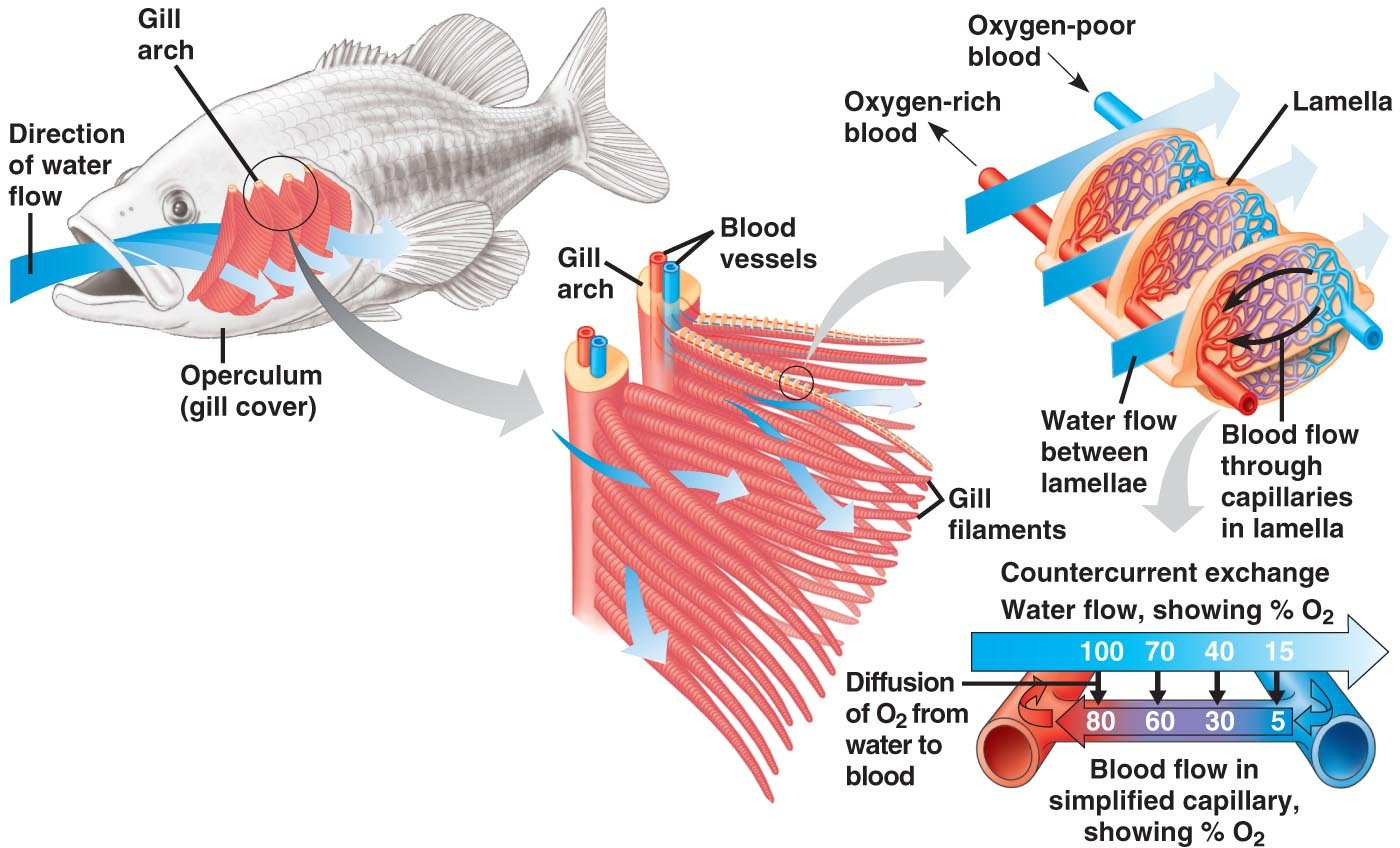
\includegraphics[width=0.618\linewidth]{./img/gills-an-o2}%
	\source{Campbell Biology}{\cite{Taylor2017}}
\end{frame}

\begin{frame}[label=current]
	\frametitle{Gill anatomy}
	\begin{tikzpicture}[remember picture,overlay]%
		\node[xshift=0,yshift=-0.0625\paperheight-0.016\paperheight/2] at (current page.center){%
			\animategraphics[autoplay,width=\paperwidth,every=2]{12}{./mov/fishhead/head-without-gills0}{001}{160}%
			};%
	\end{tikzpicture}%
\end{frame}

\begin{frame}
	\frametitle{Gill anatomy}
	\begin{tikzpicture}[remember picture,overlay]%
		\node[xshift=0,yshift=-0.0625\paperheight-0.016\paperheight/2] at (current page.center){%
			\animategraphics[autoplay,width=\paperwidth,every=\everyframe]{25}{./mov/fishhead/head-without-gills0}{161}{481}%
			};%
	\end{tikzpicture}%
\end{frame}

\begin{frame}
	\frametitle{How?}
	\begin{columns}
	\begin{column}{0.5\linewidth}
		\begin{itemize}
			\item<1-> Training for \SI{5}{w}, \SI{5}{\day\per w}, \SI{6}{\hour\per\day}, at \SI{66}{\percent} of critical speed~\cite{Palstra2010}
			\note{Comparable with the weekly training routine of Michael Phelps.
				The fish trained only for ca. \SI{7}{\percent} of their lifetime and started as adults.
				The Olympic winner trained for half of his lifetime and started as child)}
			\begin{itemize}
				\item<2-> Endurance
			\end{itemize}
			\item<3-> Morphology \& Physiology
			\begin{itemize}
				\item<3-> Body size \& weight
				\item<3-> \ce{O2} consumption
			\end{itemize}
			\item<4-> Electron microscopy
			\begin{itemize}
				\item<4-> Qualitative gill structure
			\end{itemize}
			\item<5-> \uct imaging \onslide<6->{and Delineation}
			\item<7-> Analysis
			\begin{itemize}
				\item<7-> Qualitative gill volume, structure and complexity
			\end{itemize}
		\end{itemize}
	\end{column}
	\begin{column}{0.5\linewidth}
		\only<1>{%
			\pgfmathsetlength{\imagewidth}{\imsize}%
			\pgfmathsetlength{\imagescale}{\imagewidth/1080}%
			\def\x{667}% scalebar-x starting at golden ratio of image width of 1080px = 667
			\def\y{547}% scalebar-y at 90% of image height of 608px = 547
			\begin{tikzpicture}[x=\imagescale,y=-\imagescale]%
				\node[anchor=north west, inner sep=0pt, outer sep=0pt] at (0,0) {\includegraphics[width=\imagewidth]{./mov/fishvideo/{{fishvideo_0033}}}};%
				% 69px = 30mm > 100px = 44mm > 1142px = 500mm, 228px = 100mm
				%\draw[|-|,blue] (410,188) -- (478,182) node [sloped,midway,above,fill=white,semitransparent,text opacity=1] {\SI{30}{\milli\meter} (TEMPORARY)};
				\draw[|-|,white] (\x,\y) -- (\x+228.4,\y) node [midway,above] {\(\approx\)\SI{10}{\centi\meter}};%
			\end{tikzpicture}%
			}%
		\only<2>{%
			% If you don't have the frames for the video, you can generate them as specified in ./mov/fishvideo/README.md
			\animategraphics[loop,autoplay,width=\linewidth,every=\everyframe]{25}{./mov/fishvideo/fishvideo_0}{001}{250}%
			}%
		\only<3>{\centering\Huge\faFish:\xspace\faRuler\xspace\&\xspace\faWeight}
	\only<4>{%
			\pgfmathsetlength{\imagewidth}{0.5\linewidth}%
			\pgfmathsetlength{\imagescale}{\imagewidth/794}%
			\def\x{491}% scalebar-x starting at golden ratio of image width of 794px = 491
			\def\y{458}% scalebar-y at 90% of image height of 509px = 458
			\def\shadow{4}% shadow parameter for scalebar
			\begin{tikzpicture}[x=\imagescale,y=-\imagescale]%
				\node[anchor=north west, inner sep=0pt, outer sep=0pt] at (0,0) {\includegraphics[width=\imagewidth]{./img/{{EM.c5.3}}}};%
				% 794px = 2.4111398mm > 100px = 304um > 165px = 500um, 33px = 100um
				%\draw[|-|,blue] (0,298) -- (794,298) node [sloped,midway,above,fill=white,semitransparent,text opacity=1] {\SI{2.4111398}{\milli\meter} (794px) TEMPORARY!};
				\draw[|-|] (\x+\shadow,\y+\shadow) -- (\x+165+\shadow,\y+\shadow) node [midway, above] {\SI{500}{\micro\meter}};%
				\draw[|-|,white] (\x,\y) -- (\x+165,\y) node [midway,above] {\SI{500}{\micro\meter}};%
			\end{tikzpicture}%
			\begin{tikzpicture}[x=\imagescale,y=-\imagescale]%
				\node[anchor=north west, inner sep=0pt, outer sep=0pt] at (0,0) {\includegraphics[width=\imagewidth]{./img/{{EM.s5.3}}}};%
				% 794px = 2.4111398mm > 100px = 304um > 165px = 500um, 33px = 100um
				%\draw[|-|,blue] (0,298) -- (794,298) node [sloped,midway,above,fill=white,semitransparent,text opacity=1] {\SI{2.4111398}{\milli\meter} (794px) TEMPORARY!};
				\draw[|-|] (\x+\shadow,\y+\shadow) -- (\x+165+\shadow,\y+\shadow) node [midway, above] {\SI{500}{\micro\meter}};%
				\draw[|-|,white] (\x,\y) -- (\x+165,\y) node [midway,above] {\SI{500}{\micro\meter}};%
			\end{tikzpicture}%
			}
		\only<5>{%
			\lstinputlisting[linerange={2-5,17-17,19-23,29-31,34-34,38-40,51-51,58-59}]{./logfiles/Control10/proj/Control10.log}%
			}
		\includegraphics<6>[height=0.6\textheight]{./img/CTAn}%
		\only<7>{%
			% If you don't have the frames for the video, you can generate them as specified in ./mov/coder/README.md
			\animategraphics[loop,autoplay,width=\linewidth,every=\everyframe]{25}{./mov/coder/coder-}{0}{133}%
			\source{gph.is/2nqkple}{}%
			}
		\end{column}
	\end{columns}
\end{frame}

\begin{frame}
	\frametitle{Body size}
	\centering
	\only<1>{\Huge\faRuler}
	\only<2>{% !TEX root = ..\20190605_BrukerUserMeeting.tex
% This file was created by matplotlib2tikz v0.7.4.
% And edited a bit by hand...
\begin{tikzpicture}

%\definecolor{color0}{rgb}{0.83921568627451,0,0.168627450980392}

\begin{axis}[
tuftelike,
scale only axis,
width=0.618\textwidth,
height=0.618\textheight,
%axis line style={white!80.0!black},
%legend cell align={left},
%legend style={at={(0.03,0.03)}, anchor=south west, draw=white!80.0!black},
%tick align=outside,
%x grid style={white!80.0!black},
%xmajorticks=false,
%xmin=-0.5, xmax=1.5,
%xtick style={color=white!15.0!black},
xtick={0,1},
xticklabels={Before Training,After Training},
%y grid style={white!80.0!black},
ylabel={Fish length [\si{\milli\metre}]},
%ymajorgrids,
%ymajorticks=false,
ymin=0, %ymax=36,
%ytick style={color=white!15.0!black}
]
\path [draw=black, fill=lightgray]
(axis cs:-0.396,28)
--(axis cs:-0.004,28)
--(axis cs:-0.004,31)
--(axis cs:-0.396,31)
--(axis cs:-0.396,28)
--cycle;
\path [draw=black, fill=ubRed]
(axis cs:0.004,28)
--(axis cs:0.396,28)
--(axis cs:0.396,30)
--(axis cs:0.004,30)
--(axis cs:0.004,28)
--cycle;
\path [draw=black, fill=lightgray]
(axis cs:0.604,29)
--(axis cs:0.996,29)
--(axis cs:0.996,31)
--(axis cs:0.604,31)
--(axis cs:0.604,29)
--cycle;
\path [draw=black, fill=ubRed]
(axis cs:1.004,29)
--(axis cs:1.396,29)
--(axis cs:1.396,31.25)
--(axis cs:1.004,31.25)
--(axis cs:1.004,29)
--cycle;
%\addplot [only marks, draw=lightgray, fill=lightgray]
%table{%
%x                      y
%};
%\addlegendentry{Control}
%\addplot [only marks, draw=ubRed, fill=ubRed]
%table{%
%x                      y
%};
%\addlegendentry{Swimmer}
%\draw[draw=white!25.098039215686274!black,fill=lightgray,line width=0.45pt] (axis cs:0,0) rectangle (axis cs:0,0);
%\addlegendimage{ybar,ybar legend,draw=white!25.098039215686274!black,fill=lightgray,line width=0.45pt};
%\addlegendentry{Control}

%\draw[draw=white!25.098039215686274!black,fill=ubRed,line width=0.45pt] (axis cs:0,0) rectangle (axis cs:0,0);
%\addlegendimage{ybar,ybar legend,draw=white!25.098039215686274!black,fill=ubRed,line width=0.45pt};
%\addlegendentry{Swimmer}

\addplot [black]
table {%
-0.2 28
-0.2 26
};
\addplot [black]
table {%
-0.2 31
-0.2 33
};
\addplot [black]
table {%
-0.298 26
-0.102 26
};
\addplot [black]
table {%
-0.298 33
-0.102 33
};
\addplot [black]
table {%
0.2 28
0.2 26
};
\addplot [black]
table {%
0.2 30
0.2 31
};
\addplot [black]
table {%
0.102 26
0.298 26
};
\addplot [black]
table {%
0.102 31
0.298 31
};
%\addplot [black, mark=x, mark size=2, mark options={solid,fill=white!25.098039215686274!black}, only marks]
%table {%
%0.2 34
%0.2 33.5
%};
\addplot [black]
table {%
0.8 29
0.8 26
};
\addplot [black]
table {%
0.8 31
0.8 32.5
};
\addplot [black]
table {%
0.702 26
0.898 26
};
\addplot [black]
table {%
0.702 32.5
0.898 32.5
};
\addplot [black]
table {%
1.2 29
1.2 27
};
\addplot [black]
table {%
1.2 31.25
1.2 34
};
\addplot [black]
table {%
1.102 27
1.298 27
};
\addplot [black]
table {%
1.102 34
1.298 34
};
\addplot [black]
table {%
-0.396 29.5
-0.004 29.5
};
\addplot [black]
table {%
0.004 28.75
0.396 28.75
};
\addplot [black]
table {%
0.604 29.25
0.996 29.25
};
\addplot [black]
table {%
1.004 30
1.396 30
};
\addplot [only marks, draw=black, fill=lightgray]
table{%
x                      y
-0.22060031342521 31
-0.245236518754418 30
-0.223871003317048 33
-0.10939624201412 29
-0.274897724458317 31
-0.205059135301331 31
-0.238882674781718 29
-0.190117488661186 31
-0.123317598973503 31
-0.278116687136839 31
-0.133244113732571 29
-0.127135843120074 30
-0.213507278170344 28
-0.203960176465566 27
-0.131177286704479 28
-0.152747527635252 26
-0.203582086155036 30
-0.100189527162738 28
-0.218950028284168 28
-0.150202639372291 27
};
\addplot [only marks, draw=black, fill=ubRed]
table{%
x                      y
0.113854346032678 31
0.252378116254645 34
0.132331964448894 33.5
0.2003570616139 30
0.238651243927012 30
0.299127041538144 28.5
0.264347684038305 27.5
0.27681077508769 31
0.108310112065255 29
0.273490775403975 28
0.153578707069287 28
0.121482462538081 29
0.228609682180972 29
0.155618825955878 29
0.284638557714886 28
0.181203327933185 28
0.209985585299855 27
0.204636646348004 28
0.189083298583902 26
0.268852142139038 27
};
\addplot [only marks, draw=black, fill=lightgray]
table{%
x                      y
0.816634663352161 30.5
0.837419322786742 29
0.753709719730354 31
0.797410983300676 31
0.87891939072543 31
0.776888687154181 30
0.867105405168363 29
0.785763338728563 31
0.874524329453829 31
0.835680774540802 32.5
0.735257320266947 30
0.758673324192436 29.5
0.748304341941384 29
0.775241072426728 29
0.791565126405243 26
0.709919668875317 28
0.859924032372095 28
0.773032507958662 29
0.75640009180378 29
0.873344442316737 28.5
};
\addplot [only marks, draw=black, fill=ubRed]
table{%
x                      y
1.21078086768249 30
1.27784142754473 32
1.13034434698628 33
1.25485316699418 29
1.19361850368543 34
1.20883538776136 30.5
1.28660149259921 30
1.16389798636407 31
1.12963636609952 34
1.13090338787589 31
1.18780464238979 30.5
1.27317960143181 29
1.16922342992569 31.5
1.10953777633563 29
1.25683188988071 27
1.10390096783168 30
1.19793991824718 28
1.19973718383187 30
1.27065924212501 29
};
\draw[|-|, thin, gray] (axis cs:1.2,34.34) -- (axis cs:0.2,34.34) node [midway,above] {\scriptsize * | p=\num{0.018}};
%\draw[] (axis cs:0.7,34.34) -- (axis cs:0.7,34.34);
%\node at (axis cs:0.7,34.34)[
%  scale=0.9,
%  fill=lightgray,
%  draw=black,
%  line width=0.6pt,
%  inner sep=2.2pt,
%  text=black,
%  rotate=0.0
%]{* | p=0.018};
\end{axis}

\end{tikzpicture}}
	\only<3>{% !TEX root = ..\20190605_BrukerUserMeeting.tex
% This file was created by matplotlib2tikz v0.7.4.
% And edited a bit by hand...
\begin{tikzpicture}

%\definecolor{color0}{rgb}{0.83921568627451,0,0.168627450980392}

\begin{axis}[
tuftelike,
scale only axis,
width=0.618\textwidth,
height=0.618\textheight,
%axis line style={white!80.0!black},
%legend cell align={left},
%legend style={at={(0.03,0.03)}, anchor=south west, draw=white!80.0!black},
%tick align=outside,
%x grid style={white!80.0!black},
%xmajorticks=false,
%xmin=-0.5, xmax=1.5,
%xtick style={color=white!15.0!black},
xtick={0,1},
xticklabels={Before Training,After Training},
%y grid style={white!80.0!black},
ylabel={Fish length [\si{\milli\metre}]},
%ymajorgrids,
%ymajorticks=false,
%ymin=0, %ymax=36,
%ytick style={color=white!15.0!black}
]
\path [draw=black, fill=lightgray]
(axis cs:-0.396,28)
--(axis cs:-0.004,28)
--(axis cs:-0.004,31)
--(axis cs:-0.396,31)
--(axis cs:-0.396,28)
--cycle;
\path [draw=black, fill=ubRed]
(axis cs:0.004,28)
--(axis cs:0.396,28)
--(axis cs:0.396,30)
--(axis cs:0.004,30)
--(axis cs:0.004,28)
--cycle;
\path [draw=black, fill=lightgray]
(axis cs:0.604,29)
--(axis cs:0.996,29)
--(axis cs:0.996,31)
--(axis cs:0.604,31)
--(axis cs:0.604,29)
--cycle;
\path [draw=black, fill=ubRed]
(axis cs:1.004,29)
--(axis cs:1.396,29)
--(axis cs:1.396,31.25)
--(axis cs:1.004,31.25)
--(axis cs:1.004,29)
--cycle;
%\addplot [only marks, draw=lightgray, fill=lightgray]
%table{%
%x                      y
%};
%\addlegendentry{Control}
%\addplot [only marks, draw=ubRed, fill=ubRed]
%table{%
%x                      y
%};
%\addlegendentry{Swimmer}
%\draw[draw=white!25.098039215686274!black,fill=lightgray,line width=0.45pt] (axis cs:0,0) rectangle (axis cs:0,0);
%\addlegendimage{ybar,ybar legend,draw=white!25.098039215686274!black,fill=lightgray,line width=0.45pt};
%\addlegendentry{Control}

%\draw[draw=white!25.098039215686274!black,fill=ubRed,line width=0.45pt] (axis cs:0,0) rectangle (axis cs:0,0);
%\addlegendimage{ybar,ybar legend,draw=white!25.098039215686274!black,fill=ubRed,line width=0.45pt};
%\addlegendentry{Swimmer}

\addplot [black]
table {%
-0.2 28
-0.2 26
};
\addplot [black]
table {%
-0.2 31
-0.2 33
};
\addplot [black]
table {%
-0.298 26
-0.102 26
};
\addplot [black]
table {%
-0.298 33
-0.102 33
};
\addplot [black]
table {%
0.2 28
0.2 26
};
\addplot [black]
table {%
0.2 30
0.2 31
};
\addplot [black]
table {%
0.102 26
0.298 26
};
\addplot [black]
table {%
0.102 31
0.298 31
};
%\addplot [black, mark=x, mark size=2, mark options={solid,fill=white!25.098039215686274!black}, only marks]
%table {%
%0.2 34
%0.2 33.5
%};
\addplot [black]
table {%
0.8 29
0.8 26
};
\addplot [black]
table {%
0.8 31
0.8 32.5
};
\addplot [black]
table {%
0.702 26
0.898 26
};
\addplot [black]
table {%
0.702 32.5
0.898 32.5
};
\addplot [black]
table {%
1.2 29
1.2 27
};
\addplot [black]
table {%
1.2 31.25
1.2 34
};
\addplot [black]
table {%
1.102 27
1.298 27
};
\addplot [black]
table {%
1.102 34
1.298 34
};
\addplot [black]
table {%
-0.396 29.5
-0.004 29.5
};
\addplot [black]
table {%
0.004 28.75
0.396 28.75
};
\addplot [black]
table {%
0.604 29.25
0.996 29.25
};
\addplot [black]
table {%
1.004 30
1.396 30
};
\addplot [only marks, draw=black, fill=lightgray]
table{%
x                      y
-0.22060031342521 31
-0.245236518754418 30
-0.223871003317048 33
-0.10939624201412 29
-0.274897724458317 31
-0.205059135301331 31
-0.238882674781718 29
-0.190117488661186 31
-0.123317598973503 31
-0.278116687136839 31
-0.133244113732571 29
-0.127135843120074 30
-0.213507278170344 28
-0.203960176465566 27
-0.131177286704479 28
-0.152747527635252 26
-0.203582086155036 30
-0.100189527162738 28
-0.218950028284168 28
-0.150202639372291 27
};
\addplot [only marks, draw=black, fill=ubRed]
table{%
x                      y
0.113854346032678 31
0.252378116254645 34
0.132331964448894 33.5
0.2003570616139 30
0.238651243927012 30
0.299127041538144 28.5
0.264347684038305 27.5
0.27681077508769 31
0.108310112065255 29
0.273490775403975 28
0.153578707069287 28
0.121482462538081 29
0.228609682180972 29
0.155618825955878 29
0.284638557714886 28
0.181203327933185 28
0.209985585299855 27
0.204636646348004 28
0.189083298583902 26
0.268852142139038 27
};
\addplot [only marks, draw=black, fill=lightgray]
table{%
x                      y
0.816634663352161 30.5
0.837419322786742 29
0.753709719730354 31
0.797410983300676 31
0.87891939072543 31
0.776888687154181 30
0.867105405168363 29
0.785763338728563 31
0.874524329453829 31
0.835680774540802 32.5
0.735257320266947 30
0.758673324192436 29.5
0.748304341941384 29
0.775241072426728 29
0.791565126405243 26
0.709919668875317 28
0.859924032372095 28
0.773032507958662 29
0.75640009180378 29
0.873344442316737 28.5
};
\addplot [only marks, draw=black, fill=ubRed]
table{%
x                      y
1.21078086768249 30
1.27784142754473 32
1.13034434698628 33
1.25485316699418 29
1.19361850368543 34
1.20883538776136 30.5
1.28660149259921 30
1.16389798636407 31
1.12963636609952 34
1.13090338787589 31
1.18780464238979 30.5
1.27317960143181 29
1.16922342992569 31.5
1.10953777633563 29
1.25683188988071 27
1.10390096783168 30
1.19793991824718 28
1.19973718383187 30
1.27065924212501 29
};
\draw[|-|, thin, gray] (axis cs:1.2,34.34) -- (axis cs:0.2,34.34) node [midway,above] {\scriptsize * | p=\num{0.018}};
%\draw[] (axis cs:0.7,34.34) -- (axis cs:0.7,34.34);
%\node at (axis cs:0.7,34.34)[
%  scale=0.9,
%  fill=lightgray,
%  draw=black,
%  line width=0.6pt,
%  inner sep=2.2pt,
%  text=black,
%  rotate=0.0
%]{* | p=0.018};
\end{axis}

\end{tikzpicture}}
	\note{Length of the fish was measured after anesthesia with procaine from the head to the tail fin (excluding the fin) with a precision of \SI{0.5}{\milli\metre}.}
	\note{\emph{whis}: float, sequence, or string (default = 1.5)
		As a float, determines the reach of the whiskers to the beyond the first and third quartiles.
		In other words, where IQR is the interquartile range (Q3-Q1), the upper whisker will extend to last datum less than Q3 + whis*IQR).
		Similarly, the lower whisker will extend to the first datum greater than Q1 - whis*IQR.
		Beyond the whiskers, data are considered outliers and are plotted as individual points.}
\end{frame}

\begin{frame}
	\frametitle{Body weight}
	\centering
	\only<1>{\Huge\faWeight}
	\only<2>{% !TEX root = ..\20190605_BrukerUserMeeting.tex
% This file was created by matplotlib2tikz v0.7.4.
% And edited a bit by hand...
\begin{tikzpicture}

%\definecolor{color0}{rgb}{0.83921568627451,0,0.168627450980392}

\begin{axis}[
tuftelike,
scale only axis,
width=0.618\textwidth,
height=0.618\textheight,
%axis line style={white!80.0!black},
%legend cell align={left},
%legend style={at={(0.03,0.03)}, anchor=south west, draw=white!80.0!black},
%tick align=outside,
%x grid style={white!80.0!black},
%xmajorticks=false,
%xmin=-0.5, xmax=1.5,
%xtick style={color=white!15.0!black},
xtick={0,1},
xticklabels={Before Training,After Training},
%y grid style={white!80.0!black},
ylabel={Fish weight [g]},
%ymajorgrids,
%ymajorticks=false,
ymin=0, %ymax=0.52206870848298,
%ytick style={color=white!15.0!black},
%ytick={0,0.1,0.2,0.3,0.4,0.5},
%yticklabels={0.0,0.1,0.2,0.3,0.4,0.5}
]
\path [draw=black, fill=lightgray]
(axis cs:-0.396,0.3275)
--(axis cs:-0.004,0.3275)
--(axis cs:-0.004,0.4125)
--(axis cs:-0.396,0.4125)
--(axis cs:-0.396,0.3275)
--cycle;
\path [draw=black, fill=ubRed]
(axis cs:0.004,0.3175)
--(axis cs:0.396,0.3175)
--(axis cs:0.396,0.415)
--(axis cs:0.004,0.415)
--(axis cs:0.004,0.3175)
--cycle;
\path [draw=black, fill=lightgray]
(axis cs:0.604,0.3675)
--(axis cs:0.996,0.3675)
--(axis cs:0.996,0.415)
--(axis cs:0.604,0.415)
--(axis cs:0.604,0.3675)
--cycle;
\path [draw=black, fill=ubRed]
(axis cs:1.004,0.39)
--(axis cs:1.396,0.39)
--(axis cs:1.396,0.49)
--(axis cs:1.004,0.49)
--(axis cs:1.004,0.39)
--cycle;
%\addplot [only marks, draw=lightgray, fill=lightgray]
%table{%
%x                      y
%};
%\addlegendentry{Control}
%\addplot [only marks, draw=ubRed, fill=ubRed]
%table{%
%x                      y
%};
%\addlegendentry{Swimmer}
%\draw[draw=white!25.098039215686274!black,fill=lightgray,line width=0.45pt] (axis cs:0,0) rectangle (axis cs:0,0);
%\addlegendimage{ybar,ybar legend,draw=white!25.098039215686274!black,fill=lightgray,line width=0.45pt};
%\addlegendentry{Control}

%\draw[draw=white!25.098039215686274!black,fill=ubRed,line width=0.45pt] (axis cs:0,0) rectangle (axis cs:0,0);
%\addlegendimage{ybar,ybar legend,draw=white!25.098039215686274!black,fill=ubRed,line width=0.45pt};
%\addlegendentry{Swimmer}

\addplot [black]
table {%
-0.2 0.3275
-0.2 0.3
};
\addplot [black]
table {%
-0.2 0.4125
-0.2 0.48
};
\addplot [black]
table {%
-0.298 0.3
-0.102 0.3
};
\addplot [black]
table {%
-0.298 0.48
-0.102 0.48
};
\addplot [black]
table {%
0.2 0.3175
0.2 0.3
};
\addplot [black]
table {%
0.2 0.415
0.2 0.43
};
\addplot [black]
table {%
0.102 0.3
0.298 0.3
};
\addplot [black]
table {%
0.102 0.43
0.298 0.43
};
\addplot [black]
table {%
0.8 0.3675
0.8 0.32
};
\addplot [black]
table {%
0.8 0.415
0.8 0.45
};
\addplot [black]
table {%
0.702 0.32
0.898 0.32
};
\addplot [black]
table {%
0.702 0.45
0.898 0.45
};
\addplot [black]
table {%
1.2 0.39
1.2 0.33
};
\addplot [black]
table {%
1.2 0.49
1.2 0.51
};
\addplot [black]
table {%
1.102 0.33
1.298 0.33
};
\addplot [black]
table {%
1.102 0.51
1.298 0.51
};
\addplot [black]
table {%
-0.396 0.365
-0.004 0.365
};
\addplot [black]
table {%
0.004 0.385
0.396 0.385
};
\addplot [black]
table {%
0.604 0.395
0.996 0.395
};
\addplot [black]
table {%
1.004 0.46
1.396 0.46
};
\addplot [only marks, draw=black, fill=lightgray]
table{%
x                      y
-0.27539234451004 0.48
-0.244125862543165 0.42
-0.107798058238524 0.39
-0.103841041592104 0.35
-0.230375549063795 0.38
-0.265334520323762 0.3
-0.217647253207641 0.46
-0.222554109865346 0.32
-0.246178005608581 0.35
-0.10956432288306 0.32
};
\addplot [only marks, draw=black, fill=ubRed]
table{%
x                      y
0.136694380392288 0.37
0.12280703120811 0.42
0.209108150672963 0.43
0.170775610213052 0.42
0.229019109566685 0.39
0.122898942023449 0.38
0.20647934052507 0.3
0.106680519857211 0.4
0.176917980422822 0.3
0.131556997000599 0.3
};
\addplot [only marks, draw=black, fill=lightgray]
table{%
x                      y
0.805860976646919 0.42
0.815940620789951 0.45
0.865324830497067 0.45
0.762356847386421 0.4
0.765407447890051 0.32
0.897442544923217 0.39
0.708482193721361 0.39
0.84757386305765 0.36
0.798843057020005 0.4
0.752649840297232 0.36
};
\addplot [only marks, draw=black, fill=ubRed]
table{%
x                      y
1.25611544146658 0.48
1.297298133168 0.39
1.22110846780478 0.51
1.28232435467917 0.49
1.19809152497838 0.33
1.1962619324544 0.49
1.19230885038759 0.36
1.18054884765675 0.46
1.13981809825435 0.44
};
%\draw[|-|, thin, gray] (axis cs:1.2,0.5151) -- (axis cs:0.8,0.5151) node [midway,above] {\scriptsize * | p=\num{0.041}};
%\draw[] (axis cs:1,0.5151) -- (axis cs:1,0.5151);
%\node at (axis cs:1,0.5151)[
%  scale=0.9,
%  fill=lightgray,
%  draw=black,
%  line width=0.6pt,
%  inner sep=2.2pt,
%  text=black,
%  rotate=0.0
%]{* | p=0.041};
%\draw[|-|, thin, gray] (axis cs:1.2,0.28785) -- (axis cs:0.2,0.28785) node [midway,below] {\scriptsize * | p=\num{0.011}};
%\draw[] (axis cs:0.7,0.28785) -- (axis cs:0.7,0.28785);
%\node at (axis cs:0.7,0.28785)[
%  scale=0.9,
%  fill=lightgray,
%  draw=black,
%  line width=0.6pt,
%  inner sep=2.2pt,
%  text=black,
%  rotate=0.0
%]{* | p=0.011};
\end{axis}

\end{tikzpicture}}
	\only<3>{% !TEX root = ..\20190605_BrukerUserMeeting.tex
% This file was created by matplotlib2tikz v0.7.4.
% And edited a bit by hand...
\begin{tikzpicture}

%\definecolor{color0}{rgb}{0.83921568627451,0,0.168627450980392}

\begin{axis}[
tuftelike,
scale only axis,
width=0.618\textwidth,
height=0.618\textheight,
%axis line style={white!80.0!black},
%legend cell align={left},
%legend style={at={(0.03,0.03)}, anchor=south west, draw=white!80.0!black},
%tick align=outside,
%x grid style={white!80.0!black},
%xmajorticks=false,
%xmin=-0.5, xmax=1.5,
%xtick style={color=white!15.0!black},
xtick={0,1},
xticklabels={Before Training,After Training},
%y grid style={white!80.0!black},
ylabel={Fish weight [g]},
%ymajorgrids,
%ymajorticks=false,
%ymin=0, %ymax=0.52206870848298,
%ytick style={color=white!15.0!black},
%ytick={0,0.1,0.2,0.3,0.4,0.5},
%yticklabels={0.0,0.1,0.2,0.3,0.4,0.5}
]
\path [draw=black, fill=lightgray]
(axis cs:-0.396,0.3275)
--(axis cs:-0.004,0.3275)
--(axis cs:-0.004,0.4125)
--(axis cs:-0.396,0.4125)
--(axis cs:-0.396,0.3275)
--cycle;
\path [draw=black, fill=ubRed]
(axis cs:0.004,0.3175)
--(axis cs:0.396,0.3175)
--(axis cs:0.396,0.415)
--(axis cs:0.004,0.415)
--(axis cs:0.004,0.3175)
--cycle;
\path [draw=black, fill=lightgray]
(axis cs:0.604,0.3675)
--(axis cs:0.996,0.3675)
--(axis cs:0.996,0.415)
--(axis cs:0.604,0.415)
--(axis cs:0.604,0.3675)
--cycle;
\path [draw=black, fill=ubRed]
(axis cs:1.004,0.39)
--(axis cs:1.396,0.39)
--(axis cs:1.396,0.49)
--(axis cs:1.004,0.49)
--(axis cs:1.004,0.39)
--cycle;
%\addplot [only marks, draw=lightgray, fill=lightgray]
%table{%
%x                      y
%};
%\addlegendentry{Control}
%\addplot [only marks, draw=ubRed, fill=ubRed]
%table{%
%x                      y
%};
%\addlegendentry{Swimmer}
%\draw[draw=white!25.098039215686274!black,fill=lightgray,line width=0.45pt] (axis cs:0,0) rectangle (axis cs:0,0);
%\addlegendimage{ybar,ybar legend,draw=white!25.098039215686274!black,fill=lightgray,line width=0.45pt};
%\addlegendentry{Control}

%\draw[draw=white!25.098039215686274!black,fill=ubRed,line width=0.45pt] (axis cs:0,0) rectangle (axis cs:0,0);
%\addlegendimage{ybar,ybar legend,draw=white!25.098039215686274!black,fill=ubRed,line width=0.45pt};
%\addlegendentry{Swimmer}

\addplot [black]
table {%
-0.2 0.3275
-0.2 0.3
};
\addplot [black]
table {%
-0.2 0.4125
-0.2 0.48
};
\addplot [black]
table {%
-0.298 0.3
-0.102 0.3
};
\addplot [black]
table {%
-0.298 0.48
-0.102 0.48
};
\addplot [black]
table {%
0.2 0.3175
0.2 0.3
};
\addplot [black]
table {%
0.2 0.415
0.2 0.43
};
\addplot [black]
table {%
0.102 0.3
0.298 0.3
};
\addplot [black]
table {%
0.102 0.43
0.298 0.43
};
\addplot [black]
table {%
0.8 0.3675
0.8 0.32
};
\addplot [black]
table {%
0.8 0.415
0.8 0.45
};
\addplot [black]
table {%
0.702 0.32
0.898 0.32
};
\addplot [black]
table {%
0.702 0.45
0.898 0.45
};
\addplot [black]
table {%
1.2 0.39
1.2 0.33
};
\addplot [black]
table {%
1.2 0.49
1.2 0.51
};
\addplot [black]
table {%
1.102 0.33
1.298 0.33
};
\addplot [black]
table {%
1.102 0.51
1.298 0.51
};
\addplot [black]
table {%
-0.396 0.365
-0.004 0.365
};
\addplot [black]
table {%
0.004 0.385
0.396 0.385
};
\addplot [black]
table {%
0.604 0.395
0.996 0.395
};
\addplot [black]
table {%
1.004 0.46
1.396 0.46
};
\addplot [only marks, draw=black, fill=lightgray]
table{%
x                      y
-0.27539234451004 0.48
-0.244125862543165 0.42
-0.107798058238524 0.39
-0.103841041592104 0.35
-0.230375549063795 0.38
-0.265334520323762 0.3
-0.217647253207641 0.46
-0.222554109865346 0.32
-0.246178005608581 0.35
-0.10956432288306 0.32
};
\addplot [only marks, draw=black, fill=ubRed]
table{%
x                      y
0.136694380392288 0.37
0.12280703120811 0.42
0.209108150672963 0.43
0.170775610213052 0.42
0.229019109566685 0.39
0.122898942023449 0.38
0.20647934052507 0.3
0.106680519857211 0.4
0.176917980422822 0.3
0.131556997000599 0.3
};
\addplot [only marks, draw=black, fill=lightgray]
table{%
x                      y
0.805860976646919 0.42
0.815940620789951 0.45
0.865324830497067 0.45
0.762356847386421 0.4
0.765407447890051 0.32
0.897442544923217 0.39
0.708482193721361 0.39
0.84757386305765 0.36
0.798843057020005 0.4
0.752649840297232 0.36
};
\addplot [only marks, draw=black, fill=ubRed]
table{%
x                      y
1.25611544146658 0.48
1.297298133168 0.39
1.22110846780478 0.51
1.28232435467917 0.49
1.19809152497838 0.33
1.1962619324544 0.49
1.19230885038759 0.36
1.18054884765675 0.46
1.13981809825435 0.44
};
\draw[|-|, thin, gray] (axis cs:1.2,0.5151) -- (axis cs:0.8,0.5151) node [midway,above] {\scriptsize * | p=\num{0.041}};
%\draw[] (axis cs:1,0.5151) -- (axis cs:1,0.5151);
%\node at (axis cs:1,0.5151)[
%  scale=0.9,
%  fill=lightgray,
%  draw=black,
%  line width=0.6pt,
%  inner sep=2.2pt,
%  text=black,
%  rotate=0.0
%]{* | p=0.041};
\draw[|-|, thin, gray] (axis cs:1.2,0.28785) -- (axis cs:0.2,0.28785) node [midway,below] {\scriptsize * | p=\num{0.011}};
%\draw[] (axis cs:0.7,0.28785) -- (axis cs:0.7,0.28785);
%\node at (axis cs:0.7,0.28785)[
%  scale=0.9,
%  fill=lightgray,
%  draw=black,
%  line width=0.6pt,
%  inner sep=2.2pt,
%  text=black,
%  rotate=0.0
%]{* | p=0.011};
\end{axis}

\end{tikzpicture}}
	\note{Weight of the fish was taken from living fish (only from males), measuring the weight of a water tank without and with fish inside.}
\end{frame}

\begin{frame}
	\frametitle{Endurance}
	\centering
	\only<1>{\Huge\faTachometer*}
	\only<2>{% !TEX root = ..\20190605_BrukerUserMeeting.tex
% This file was created by matplotlib2tikz v0.7.4.
% And edited a bit by hand...
\begin{tikzpicture}

%\definecolor{color0}{rgb}{0.83921568627451,0,0.168627450980392}

\begin{axis}[
tuftelike,
scale only axis,
width=0.618\textwidth,
height=0.618\textheight,
%axis line style={white!80.0!black},
%legend cell align={left},
%legend style={at={(0.03,0.03)}, anchor=south west, draw=white!80.0!black},
%tick align=outside,
%x grid style={white!80.0!black},
%xmajorticks=false,
%xmin=-0.5, xmax=1.5,
%xtick style={color=white!15.0!black},
xtick={0,1},
xticklabels={Before Training,After Training},
%y grid style={white!80.0!black},
ylabel={Water current speed [\si{\centi\metre\per\second}]},
%ymajorgrids,
%ymajorticks=false,
ymin=0, %ymax=51.4367510098786,
%ytick style={color=white!15.0!black}
]
\path [draw=black, fill=lightgray]
(axis cs:-0.396,30)
--(axis cs:-0.004,30)
--(axis cs:-0.004,40)
--(axis cs:-0.396,40)
--(axis cs:-0.396,30)
--cycle;
\path [draw=black, fill=ubRed]
(axis cs:0.004,30)
--(axis cs:0.396,30)
--(axis cs:0.396,40)
--(axis cs:0.004,40)
--(axis cs:0.004,30)
--cycle;
\path [draw=black, fill=lightgray]
(axis cs:0.604,33.75)
--(axis cs:0.996,33.75)
--(axis cs:0.996,40)
--(axis cs:0.604,40)
--(axis cs:0.604,33.75)
--cycle;
\path [draw=black, fill=ubRed]
(axis cs:1.004,40)
--(axis cs:1.396,40)
--(axis cs:1.396,47.5)
--(axis cs:1.004,47.5)
--(axis cs:1.004,40)
--cycle;
%\addplot [only marks, draw=lightgray, fill=lightgray]
%table{%
%x                      y
%};
%\addlegendentry{Control}
%\addplot [only marks, draw=ubRed, fill=ubRed]
%table{%
%x                      y
%};
%\addlegendentry{Swimmer}
%\draw[draw=white!25.098039215686274!black,fill=lightgray,line width=0.45pt] (axis cs:0,0) rectangle (axis cs:0,0);
%\addlegendimage{ybar,ybar legend,draw=white!25.098039215686274!black,fill=lightgray,line width=0.45pt};
%\addlegendentry{Control}

%\draw[draw=white!25.098039215686274!black,fill=ubRed,line width=0.45pt] (axis cs:0,0) rectangle (axis cs:0,0);
%\addlegendimage{ybar,ybar legend,draw=white!25.098039215686274!black,fill=ubRed,line width=0.45pt};
%\addlegendentry{Swimmer}

\addplot [black]
table {%
-0.2 30
-0.2 25
};
\addplot [black]
table {%
-0.2 40
-0.2 40
};
\addplot [black]
table {%
-0.298 25
-0.102 25
};
\addplot [black]
table {%
-0.298 40
-0.102 40
};
\addplot [black]
table {%
0.2 30
0.2 25
};
\addplot [black]
table {%
0.2 40
0.2 40
};
\addplot [black]
table {%
0.102 25
0.298 25
};
\addplot [black]
table {%
0.102 40
0.298 40
};
\addplot [black]
table {%
0.8 33.75
0.8 30
};
\addplot [black]
table {%
0.8 40
0.8 45
};
\addplot [black]
table {%
0.702 30
0.898 30
};
\addplot [black]
table {%
0.702 45
0.898 45
};
\addplot [black]
table {%
1.2 40
1.2 35
};
\addplot [black]
table {%
1.2 47.5
1.2 50
};
\addplot [black]
table {%
1.102 35
1.298 35
};
\addplot [black]
table {%
1.102 50
1.298 50
};
\addplot [black]
table {%
-0.396 35
-0.004 35
};
\addplot [black]
table {%
0.004 30
0.396 30
};
\addplot [black]
table {%
0.604 35
0.996 35
};
\addplot [black]
table {%
1.004 45
1.396 45
};
\addplot [only marks, draw=black, fill=lightgray]
table{%
x                      y
-0.164969508708635 25
-0.250249527025853 25
-0.191393326546884 30
-0.238532832844393 30
-0.240084042030871 35
-0.167719712630741 30
-0.177156001637211 30
-0.273093850638075 30
-0.230057169680332 35
-0.199330773439484 35
-0.121684893668749 40
-0.158116604896962 40
-0.236906056649543 40
-0.125386242161757 40
-0.101945401835971 40
-0.106388945743883 40
-0.149125487165791 40
-0.261511500828116 35
-0.231757957079711 35
-0.188448469900678 30
};
\addplot [only marks, draw=black, fill=ubRed]
table{%
x                      y
0.265771032632614 30
0.171203566873329 25
0.249471402169787 30
0.298454878631275 30
0.215196091954096 30
0.264492058277436 30
0.228142876769728 30
0.135984625151926 25
0.144578795486409 25
0.234600459190529 30
0.19625884342528 40
0.205096637453532 40
0.280511880213459 40
0.211052994798684 40
0.29231913668364 40
0.108584526449881 40
0.11223052287585 40
0.18050056432311 35
0.233341893743106 35
0.222970985087893 30
};
\addplot [only marks, draw=black, fill=lightgray]
table{%
x                      y
0.845103613735034 30
0.859995829395603 30
0.819765799704493 30
0.723660017978818 30
0.780216167167552 35
0.794504145509713 35
0.705102679190906 35
0.875063282610662 35
0.856890965504197 30
0.831367768058273 35
0.741690666845684 45
0.898073778373665 40
0.775060309925967 35
0.739744637260933 40
0.749075296023897 40
0.742799820558281 40
0.781666246403571 45
0.750159728497048 35
0.703999680626644 40
0.891773742857554 35
};
\addplot [only marks, draw=black, fill=ubRed]
table{%
x                      y
1.16839196661205 45
1.22047053375793 40
1.11207438813402 35
1.24750859090223 40
1.14868318655751 40
1.14607352138115 40
1.14435276995225 40
1.2131823970255 45
1.12079342556317 40
1.24955612610569 40
1.2119957533795 50
1.28246481702868 50
1.12518724319397 50
1.14843470488118 50
1.26815664128491 45
1.19247136453775 50
1.21335277635983 45
1.287249560505 45
1.27655898312702 45
};
\draw[|-|, thin, gray] (axis cs:1.2,50.5) -- (axis cs:0.8,50.5) node [midway,above] {\scriptsize *** | p=\num{2.7e-06}};
%\draw[] (axis cs:1,50.5) -- (axis cs:1,50.5);
%\node at (axis cs:1,50.5)[
%  scale=0.9,
%  fill=lightgray,
%  draw=black,
%  line width=0.6pt,
%  inner sep=2.2pt,
%  text=black,
%  rotate=0.0
%]{*** | p=2.7e-06};
\draw[|-|, thin, gray] (axis cs:1.2,23.9875) -- (axis cs:0.2,23.9875) node [midway,below] {\scriptsize *** | p=\num{7.8e-08}};
%\draw[] (axis cs:0.7,23.9875) -- (axis cs:0.7,23.9875);
%\node at (axis cs:0.7,23.9875)[
%  scale=0.9,
%  fill=lightgray,
%  draw=black,
%  line width=0.6pt,
%  inner sep=2.2pt,
%  text=black,
%  rotate=0.0
%]{*** | p=7.8e-08};
\end{axis}

\end{tikzpicture}}
	\only<3>{% !TEX root = ..\20190605_BrukerUserMeeting.tex
% This file was created by matplotlib2tikz v0.7.4.
% And edited a bit by hand...
\begin{tikzpicture}

%\definecolor{color0}{rgb}{0.83921568627451,0,0.168627450980392}

\begin{axis}[
simplified,
scale only axis,
width=0.75\textwidth,
height=.618\textheight,
%axis line style={white!80.0!black},
%legend cell align={left},
%legend style={at={(0.03,0.03)}, anchor=south west, draw=white!80.0!black},
%tick align=outside,
%x grid style={white!80.0!black},
%xmajorticks=false,
%xmin=-0.5, xmax=1.5,
%xtick style={color=white!15.0!black},
xtick={0,1},
xticklabels={Before Training,After Training},
%y grid style={white!80.0!black},
ylabel={Water current speed [\si{\centi\metre\per\second}]},
%ymajorgrids,
%ymajorticks=false,
ymin=21.6,
%ymax=51.4367510098786,
%ytick style={color=white!15.0!black}
]
\path [draw=black, fill=lightgray]
(axis cs:-0.396,30)
--(axis cs:-0.004,30)
--(axis cs:-0.004,40)
--(axis cs:-0.396,40)
--(axis cs:-0.396,30)
--cycle;
\path [draw=black, fill=ubRed]
(axis cs:0.004,30)
--(axis cs:0.396,30)
--(axis cs:0.396,40)
--(axis cs:0.004,40)
--(axis cs:0.004,30)
--cycle;
\path [draw=black, fill=lightgray]
(axis cs:0.604,33.75)
--(axis cs:0.996,33.75)
--(axis cs:0.996,40)
--(axis cs:0.604,40)
--(axis cs:0.604,33.75)
--cycle;
\path [draw=black, fill=ubRed]
(axis cs:1.004,40)
--(axis cs:1.396,40)
--(axis cs:1.396,47.5)
--(axis cs:1.004,47.5)
--(axis cs:1.004,40)
--cycle;
%\addplot [only marks, draw=lightgray, fill=lightgray]
%table{%
%x                      y
%};
%\addlegendentry{Control}
%\addplot [only marks, draw=ubRed, fill=ubRed]
%table{%
%x                      y
%};
%\addlegendentry{Swimmer}
%\draw[draw=white!25.098039215686274!black,fill=lightgray,line width=0.45pt] (axis cs:0,0) rectangle (axis cs:0,0);
%\addlegendimage{ybar,ybar legend,draw=white!25.098039215686274!black,fill=lightgray,line width=0.45pt};
%\addlegendentry{Control}

%\draw[draw=white!25.098039215686274!black,fill=ubRed,line width=0.45pt] (axis cs:0,0) rectangle (axis cs:0,0);
%\addlegendimage{ybar,ybar legend,draw=white!25.098039215686274!black,fill=ubRed,line width=0.45pt};
%\addlegendentry{Swimmer}

\addplot [black]
table {%
-0.2 30
-0.2 25
};
\addplot [black]
table {%
-0.2 40
-0.2 40
};
\addplot [black]
table {%
-0.298 25
-0.102 25
};
\addplot [black]
table {%
-0.298 40
-0.102 40
};
\addplot [black]
table {%
0.2 30
0.2 25
};
\addplot [black]
table {%
0.2 40
0.2 40
};
\addplot [black]
table {%
0.102 25
0.298 25
};
\addplot [black]
table {%
0.102 40
0.298 40
};
\addplot [black]
table {%
0.8 33.75
0.8 30
};
\addplot [black]
table {%
0.8 40
0.8 45
};
\addplot [black]
table {%
0.702 30
0.898 30
};
\addplot [black]
table {%
0.702 45
0.898 45
};
\addplot [black]
table {%
1.2 40
1.2 35
};
\addplot [black]
table {%
1.2 47.5
1.2 50
};
\addplot [black]
table {%
1.102 35
1.298 35
};
\addplot [black]
table {%
1.102 50
1.298 50
};
\addplot [black]
table {%
-0.396 35
-0.004 35
};
\addplot [black]
table {%
0.004 30
0.396 30
};
\addplot [black]
table {%
0.604 35
0.996 35
};
\addplot [black]
table {%
1.004 45
1.396 45
};
\addplot [only marks, draw=black, fill=lightgray]
table{%
x                      y
-0.164969508708635 25
-0.250249527025853 25
-0.191393326546884 30
-0.238532832844393 30
-0.240084042030871 35
-0.167719712630741 30
-0.177156001637211 30
-0.273093850638075 30
-0.230057169680332 35
-0.199330773439484 35
-0.121684893668749 40
-0.158116604896962 40
-0.236906056649543 40
-0.125386242161757 40
-0.101945401835971 40
-0.106388945743883 40
-0.149125487165791 40
-0.261511500828116 35
-0.231757957079711 35
-0.188448469900678 30
};
\addplot [only marks, draw=black, fill=ubRed]
table{%
x                      y
0.265771032632614 30
0.171203566873329 25
0.249471402169787 30
0.298454878631275 30
0.215196091954096 30
0.264492058277436 30
0.228142876769728 30
0.135984625151926 25
0.144578795486409 25
0.234600459190529 30
0.19625884342528 40
0.205096637453532 40
0.280511880213459 40
0.211052994798684 40
0.29231913668364 40
0.108584526449881 40
0.11223052287585 40
0.18050056432311 35
0.233341893743106 35
0.222970985087893 30
};
\addplot [only marks, draw=black, fill=lightgray]
table{%
x                      y
0.845103613735034 30
0.859995829395603 30
0.819765799704493 30
0.723660017978818 30
0.780216167167552 35
0.794504145509713 35
0.705102679190906 35
0.875063282610662 35
0.856890965504197 30
0.831367768058273 35
0.741690666845684 45
0.898073778373665 40
0.775060309925967 35
0.739744637260933 40
0.749075296023897 40
0.742799820558281 40
0.781666246403571 45
0.750159728497048 35
0.703999680626644 40
0.891773742857554 35
};
\addplot [only marks, draw=black, fill=ubRed]
table{%
x                      y
1.16839196661205 45
1.22047053375793 40
1.11207438813402 35
1.24750859090223 40
1.14868318655751 40
1.14607352138115 40
1.14435276995225 40
1.2131823970255 45
1.12079342556317 40
1.24955612610569 40
1.2119957533795 50
1.28246481702868 50
1.12518724319397 50
1.14843470488118 50
1.26815664128491 45
1.19247136453775 50
1.21335277635983 45
1.287249560505 45
1.27655898312702 45
};
\draw[|-|, thin, gray] (axis cs:1.2,50.5) -- (axis cs:0.8,50.5) node [midway,above] {\scriptsize *** | p=\num{2.7e-06}};
%\draw[] (axis cs:1,50.5) -- (axis cs:1,50.5);
%\node at (axis cs:1,50.5)[
%  scale=0.9,
%  fill=lightgray,
%  draw=black,
%  line width=0.6pt,
%  inner sep=2.2pt,
%  text=black,
%  rotate=0.0
%]{*** | p=2.7e-06};
\draw[|-|, thin, gray] (axis cs:1.2,23.9875) -- (axis cs:0.2,23.9875) node [midway,below] {\scriptsize *** | p=\num{7.8e-08}};
%\draw[] (axis cs:0.7,23.9875) -- (axis cs:0.7,23.9875);
%\node at (axis cs:0.7,23.9875)[
%  scale=0.9,
%  fill=lightgray,
%  draw=black,
%  line width=0.6pt,
%  inner sep=2.2pt,
%  text=black,
%  rotate=0.0
%]{*** | p=7.8e-08};
\end{axis}

\end{tikzpicture}}
\end{frame}

\begin{frame}
	\frametitle{Gill structure}
	\centering
	\only<1>{%
		\pgfmathsetlength{\imagewidth}{0.5\linewidth}%
		\pgfmathsetlength{\imagescale}{\imagewidth/794}%
		\def\x{491}% scalebar-x starting at golden ratio of image width of 794px = 491
		\def\y{458}% scalebar-y at 90% of image height of 509px = 458
		\def\shadow{4}% shadow parameter for scalebar
		\begin{tikzpicture}[x=\imagescale,y=-\imagescale]%
			\node[anchor=north west, inner sep=0pt, outer sep=0pt] at (0,0) {\includegraphics[width=\imagewidth]{./img/{{EM.c5.3}}}};%
			% 794px = 2.4111398mm > 100px = 304um > 165px = 500um, 33px = 100um
			%\draw[|-|,blue] (0,298) -- (794,298) node [sloped,midway,above,fill=white,semitransparent,text opacity=1] {\SI{2.4111398}{\milli\meter} (794px) TEMPORARY!};
			\draw[|-|] (\x+\shadow,\y+\shadow) -- (\x+165+\shadow,\y+\shadow) node [midway, above] {\SI{500}{\micro\meter}};%
			\draw[|-|,white] (\x,\y) -- (\x+165,\y) node [midway,above] {\SI{500}{\micro\meter}};%
		\end{tikzpicture}%
		\begin{tikzpicture}[x=\imagescale,y=-\imagescale]%
			\node[anchor=north west, inner sep=0pt, outer sep=0pt] at (0,0) {\includegraphics[width=\imagewidth]{./img/{{EM.s5.3}}}};%
			% 794px = 2.4111398mm > 100px = 304um > 165px = 500um, 33px = 100um
			%\draw[|-|,blue] (0,298) -- (794,298) node [sloped,midway,above,fill=white,semitransparent,text opacity=1] {\SI{2.4111398}{\milli\meter} (794px) TEMPORARY!};
			\draw[|-|] (\x+\shadow,\y+\shadow) -- (\x+165+\shadow,\y+\shadow) node [midway, above] {\SI{500}{\micro\meter}};%
			\draw[|-|,white] (\x,\y) -- (\x+165,\y) node [midway,above] {\SI{500}{\micro\meter}};%
		\end{tikzpicture}%
		}
	\only<2>{% !TEX root = ..\20190605_BrukerUserMeeting.tex
% This file was created by matplotlib2tikz v0.7.4.
% And edited a bit by hand...
\begin{tikzpicture}

%\definecolor{color0}{rgb}{0.83921568627451,0,0.168627450980392}

\begin{axis}[
tuftelike,
scale only axis,
width=0.618\textwidth,
height=0.618\textheight,
%axis line style={white!80.0!black},
%tick align=outside,
%x grid style={white!80.0!black},
%xmajorticks=false,
%xmin=-0.5, xmax=1.5,
%xtick style={color=white!15.0!black},
xtick={0,1},
xticklabels={Control,Swimmer},
%y grid style={white!80.0!black},
ylabel={Primary filament length [\si{\micro\metre}]},
%ymajorgrids,
%ymajorticks=false,
ymin=0, %ymax=2176.41222712779,
%ytick style={color=white!15.0!black}
]
\path [draw=black, fill=lightgray]
(axis cs:-0.4,1432.08333333333)
--(axis cs:0.4,1432.08333333333)
--(axis cs:0.4,1693.66666666667)
--(axis cs:-0.4,1693.66666666667)
--(axis cs:-0.4,1432.08333333333)
--cycle;
\path [draw=black, fill=ubRed]
(axis cs:0.6,1445.20833333333)
--(axis cs:1.4,1445.20833333333)
--(axis cs:1.4,1824.41666666667)
--(axis cs:0.6,1824.41666666667)
--(axis cs:0.6,1445.20833333333)
--cycle;
\addplot [black]
table {%
0 1432.08333333333
0 1211.66666666667
};
\addplot [black]
table {%
0 1693.66666666667
0 1798.33333333333
};
\addplot [black]
table {%
-0.2 1211.66666666667
0.2 1211.66666666667
};
\addplot [black]
table {%
-0.2 1798.33333333333
0.2 1798.33333333333
};
\addplot [black]
table {%
1 1445.20833333333
1 1202
};
\addplot [black]
table {%
1 1824.41666666667
1 2123.5
};
\addplot [black]
table {%
0.8 1202
1.2 1202
};
\addplot [black]
table {%
0.8 2123.5
1.2 2123.5
};
\addplot [black]
table {%
-0.4 1509.66666666667
0.4 1509.66666666667
};
\addplot [black]
table {%
0.6 1617.5
1.4 1617.5
};
\addplot [only marks, draw=black, fill=lightgray]
table{%
x                      y
-0.174116852372548 1777.33333333333
0.00526365359063008 1739
0.0896225022645724 1717.33333333333
0.138817648332402 1728.5
0.169147630700476 1714.16666666667
0.187209016888342 1708.83333333333
0.0695145544723801 1712.5
0.187812776534036 1675.5
0.1548193814982 1667.16666666667
-0.179322577690997 1653.16666666667
0.166967851884652 1585.5
-0.19879365760715 1602.33333333333
-0.173880390946597 1449.66666666667
-0.0723922256512002 1395.66666666667
0.154741286237046 1211.66666666667
0.179895955069079 1726.33333333333
0.0197434692178516 1505.33333333333
-0.136962715726775 1626.83333333333
-0.0423855724261894 1482.83333333333
-0.136254747189248 1375
-0.0925593715228482 1727.33333333333
-0.050133017054345 1768.33333333333
-0.0654815860072047 1721.83333333333
0.0246084161426108 1769.33333333333
-0.148642116412848 1719.33333333333
-0.0278201380683009 1461.33333333333
0.0925568143340804 1593
0.00271904515615778 1509.66666666667
0.0206339033737981 1595
-0.141737605082689 1516.66666666667
0.147080992161849 1694.33333333333
-0.198437580442956 1679.16666666667
0.156010670015503 1495
0.111335313451597 1433.66666666667
-0.00175917220546101 1479
0.199905713650341 1553
-0.0771625215537039 1615.33333333333
-0.0218631449191333 1625
0.117019142572137 1593.5
-0.0534096672312082 1371.33333333333
-0.187489071554163 1625.16666666667
-0.116940731144452 1725
-0.167565347516652 1651.33333333333
-0.0671499350524119 1588.5
-0.048578100844953 1430.5
-0.197482212525957 1405.33333333333
-0.0467676789487931 1422.33333333333
0.187598804715712 1415.16666666667
0.0590308846540935 1503.5
0.0669935383487654 1478.33333333333
-0.123201687405394 1361.66666666667
0.0188734578867463 1512.83333333333
-0.0970335487461247 1395.5
0.100605903605678 1410.16666666667
-0.0575553811094791 1385.66666666667
-0.16399302396832 1333.83333333333
0.0168235277743853 1418
-0.0463892150127354 1479.66666666667
0.164085613708626 1279
0.153067651593879 1295.83333333333
-0.184205107412278 1247.33333333333
-0.111700946725676 1382.83333333333
0.0865727259479874 1424.5
0.0979615606962427 1376
-0.0770459356660075 1473.83333333333
0.0660088665434571 1647.16666666667
0.0312931737584829 1730.66666666667
0.0385562392438058 1761
0.0314926691594624 1778
0.0872633210052943 1693
0.161242765847361 1731.83333333333
0.170222843194104 1593.16666666667
0.0369733909756579 1507.16666666667
-0.0739117313514655 1532.66666666667
-0.0930661413160724 1536.83333333333
-0.101662516871052 1472.16666666667
-0.173319289713967 1465.16666666667
-0.0927352101354389 1459.83333333333
-0.0368621765419722 1497
-0.120396606087295 1453.5
-0.085315307905426 1371.33333333333
0.0926124782358558 1338.66666666667
0.139692004940519 1327.33333333333
0.0646244586180719 1455.83333333333
0.171964067143942 1340.83333333333
-0.000544579584789734 1712
0.0308940627568505 1696
0.0822582642539244 1764.5
0.159392840036499 1798.33333333333
0.169588772909538 1774.33333333333
-0.00080543332463931 1442
-0.159192274482471 1455.5
-0.0119668084364619 1506.33333333333
0.126133409074429 1472.83333333333
0.0367412876210591 1465.33333333333
};
\addplot [only marks, draw=black, fill=ubRed]
table{%
x                      y
0.942846892581578 1364.83333333333
1.11629342266704 1464
1.00634893534917 1408.16666666667
1.12317792931768 1417.33333333333
1.17690478080561 1295
1.19759148085446 1434.66666666667
1.17035440802526 1516
0.81260919984559 1562
0.866940660746269 1547.16666666667
1.10580618376161 1468.66666666667
1.15274260047369 1619.66666666667
1.16605339840564 1708.5
1.16048415896893 1671.83333333333
1.12894772753524 1655.66666666667
1.04880862651024 1595.83333333333
0.865903038406308 1644.66666666667
1.1801395468171 1608.5
0.944479746559962 1669.83333333333
0.868322363609166 1724.5
0.922950648929207 1685.66666666667
0.921821757596963 1827.66666666667
1.12510545250631 1878.16666666667
1.18366148434612 2013.66666666667
0.891982414930724 1961.5
0.800822571767133 1915
0.836230593042283 1852
0.822299811577936 1874.66666666667
1.04164744790137 1681.5
0.920572353219958 2041.33333333333
1.18419422400489 1681.66666666667
0.969796039883939 1618.16666666667
0.861830470759354 1445.83333333333
1.04188435389371 1398
1.1816477484353 1202
0.998650273802606 1337.16666666667
0.939674687753346 1394.5
1.19230978429752 1312.16666666667
1.15464118821129 1322
1.00561508018277 1320.66666666667
0.904396096454412 1307.66666666667
0.967250649099106 1942.83333333333
0.870034734811856 1937.66666666667
1.15531795493121 1927.33333333333
1.10844082337526 1936.5
1.17103328851795 1934.5
0.959155465666125 1842.5
0.832939599291264 2019
1.1724768462939 2034.5
0.9208560994309 2008.66666666667
1.19791712404957 1803.66666666667
0.855059930700466 1616.83333333333
0.878399980876992 1611
1.05994148052408 1553.66666666667
0.958472412009966 1523.83333333333
0.925844446601199 1532.5
0.803016754969765 1566
1.1513006633981 1429.83333333333
1.07746862887688 1449.33333333333
0.94507447854429 1512.33333333333
0.861607969575037 1448.66666666667
1.13860665670348 1735.66666666667
1.08189645997604 1849
1.1190528026322 1860.33333333333
1.01760235747267 1724.5
1.08482995508157 1653.66666666667
0.819398574728977 1743.83333333333
0.801167159056257 1809.16666666667
0.938856025734591 1723.33333333333
0.932869576040269 1811.83333333333
1.00984127205838 1823.33333333333
0.97081218902693 1443.33333333333
1.0532540455747 1461.33333333333
0.939062880558463 1470
0.947247067355966 1418.16666666667
1.03353901652207 1416.33333333333
1.13059100076841 1357.83333333333
1.17094318675194 1451.66666666667
1.11970340698576 1537.33333333333
0.895029452164656 1432.33333333333
0.868785877780455 1367.83333333333
1.14574574241585 2123.5
1.1936674162731 2122.66666666667
0.98836946676292 2014.16666666667
1.02519746518951 1993
1.11522917837871 1942.33333333333
0.833926123845064 1780.16666666667
0.960968569676939 1774.16666666667
0.832097549656784 1742.83333333333
0.826928862430085 1871
1.17256518651408 1735.33333333333
1.02680768823101 1596.83333333333
1.12212762428404 1618.33333333333
1.16893705094204 1564.5
1.08731835679472 1528
1.0380375245373 1475.33333333333
0.987907103477216 1349.83333333333
1.0591263950515 1418.33333333333
0.922952195183012 1443.33333333333
1.09870184001454 1288.66666666667
1.08639466613256 1310.16666666667
};
%\draw[|-|, thin, gray] (axis cs:1,2144.735) -- (axis cs:0,2144.735) node [midway,above] {\scriptsize *** | p=\num{0.00043}};
%\draw[] (axis cs:0.5,2144.735) -- (axis cs:0.5,2144.735);
%\node at (axis cs:0.5,2144.735)[
%  scale=0.9,
%  fill=lightgray,
%  draw=black,
%  line width=0.6pt,
%  inner sep=2.2pt,
%  text=black,
%  rotate=0.0
%]{*** | p=0.00043};
\end{axis}

\end{tikzpicture}}
	\only<3>{% !TEX root = ..\20190605_BrukerUserMeeting.tex
% This file was created by matplotlib2tikz v0.7.4.
% And edited a bit by hand...
\begin{tikzpicture}

%\definecolor{color0}{rgb}{0.83921568627451,0,0.168627450980392}

\begin{axis}[
simplified,
scale only axis,
width=0.75\textwidth,
height=.618\textheight,
%axis line style={white!80.0!black},
%tick align=outside,
%x grid style={white!80.0!black},
%xmajorticks=false,
%xmin=-0.5, xmax=1.5,
%xtick style={color=white!15.0!black},
xtick={0,1},
xticklabels={Control,Swimmer},
%y grid style={white!80.0!black},
ylabel={Primary filament length [\si{\micro\metre}]},
%ymajorgrids,
%ymajorticks=false,
%ymin=0, %ymax=2176.41222712779,
%ytick style={color=white!15.0!black}
]
\path [draw=black, fill=lightgray]
(axis cs:-0.4,1432.08333333333)
--(axis cs:0.4,1432.08333333333)
--(axis cs:0.4,1693.66666666667)
--(axis cs:-0.4,1693.66666666667)
--(axis cs:-0.4,1432.08333333333)
--cycle;
\path [draw=black, fill=ubRed]
(axis cs:0.6,1445.20833333333)
--(axis cs:1.4,1445.20833333333)
--(axis cs:1.4,1824.41666666667)
--(axis cs:0.6,1824.41666666667)
--(axis cs:0.6,1445.20833333333)
--cycle;
\addplot [black]
table {%
0 1432.08333333333
0 1211.66666666667
};
\addplot [black]
table {%
0 1693.66666666667
0 1798.33333333333
};
\addplot [black]
table {%
-0.2 1211.66666666667
0.2 1211.66666666667
};
\addplot [black]
table {%
-0.2 1798.33333333333
0.2 1798.33333333333
};
\addplot [black]
table {%
1 1445.20833333333
1 1202
};
\addplot [black]
table {%
1 1824.41666666667
1 2123.5
};
\addplot [black]
table {%
0.8 1202
1.2 1202
};
\addplot [black]
table {%
0.8 2123.5
1.2 2123.5
};
\addplot [black]
table {%
-0.4 1509.66666666667
0.4 1509.66666666667
};
\addplot [black]
table {%
0.6 1617.5
1.4 1617.5
};
\addplot [only marks, draw=black, fill=lightgray]
table{%
x                      y
-0.174116852372548 1777.33333333333
0.00526365359063008 1739
0.0896225022645724 1717.33333333333
0.138817648332402 1728.5
0.169147630700476 1714.16666666667
0.187209016888342 1708.83333333333
0.0695145544723801 1712.5
0.187812776534036 1675.5
0.1548193814982 1667.16666666667
-0.179322577690997 1653.16666666667
0.166967851884652 1585.5
-0.19879365760715 1602.33333333333
-0.173880390946597 1449.66666666667
-0.0723922256512002 1395.66666666667
0.154741286237046 1211.66666666667
0.179895955069079 1726.33333333333
0.0197434692178516 1505.33333333333
-0.136962715726775 1626.83333333333
-0.0423855724261894 1482.83333333333
-0.136254747189248 1375
-0.0925593715228482 1727.33333333333
-0.050133017054345 1768.33333333333
-0.0654815860072047 1721.83333333333
0.0246084161426108 1769.33333333333
-0.148642116412848 1719.33333333333
-0.0278201380683009 1461.33333333333
0.0925568143340804 1593
0.00271904515615778 1509.66666666667
0.0206339033737981 1595
-0.141737605082689 1516.66666666667
0.147080992161849 1694.33333333333
-0.198437580442956 1679.16666666667
0.156010670015503 1495
0.111335313451597 1433.66666666667
-0.00175917220546101 1479
0.199905713650341 1553
-0.0771625215537039 1615.33333333333
-0.0218631449191333 1625
0.117019142572137 1593.5
-0.0534096672312082 1371.33333333333
-0.187489071554163 1625.16666666667
-0.116940731144452 1725
-0.167565347516652 1651.33333333333
-0.0671499350524119 1588.5
-0.048578100844953 1430.5
-0.197482212525957 1405.33333333333
-0.0467676789487931 1422.33333333333
0.187598804715712 1415.16666666667
0.0590308846540935 1503.5
0.0669935383487654 1478.33333333333
-0.123201687405394 1361.66666666667
0.0188734578867463 1512.83333333333
-0.0970335487461247 1395.5
0.100605903605678 1410.16666666667
-0.0575553811094791 1385.66666666667
-0.16399302396832 1333.83333333333
0.0168235277743853 1418
-0.0463892150127354 1479.66666666667
0.164085613708626 1279
0.153067651593879 1295.83333333333
-0.184205107412278 1247.33333333333
-0.111700946725676 1382.83333333333
0.0865727259479874 1424.5
0.0979615606962427 1376
-0.0770459356660075 1473.83333333333
0.0660088665434571 1647.16666666667
0.0312931737584829 1730.66666666667
0.0385562392438058 1761
0.0314926691594624 1778
0.0872633210052943 1693
0.161242765847361 1731.83333333333
0.170222843194104 1593.16666666667
0.0369733909756579 1507.16666666667
-0.0739117313514655 1532.66666666667
-0.0930661413160724 1536.83333333333
-0.101662516871052 1472.16666666667
-0.173319289713967 1465.16666666667
-0.0927352101354389 1459.83333333333
-0.0368621765419722 1497
-0.120396606087295 1453.5
-0.085315307905426 1371.33333333333
0.0926124782358558 1338.66666666667
0.139692004940519 1327.33333333333
0.0646244586180719 1455.83333333333
0.171964067143942 1340.83333333333
-0.000544579584789734 1712
0.0308940627568505 1696
0.0822582642539244 1764.5
0.159392840036499 1798.33333333333
0.169588772909538 1774.33333333333
-0.00080543332463931 1442
-0.159192274482471 1455.5
-0.0119668084364619 1506.33333333333
0.126133409074429 1472.83333333333
0.0367412876210591 1465.33333333333
};
\addplot [only marks, draw=black, fill=ubRed]
table{%
x                      y
0.942846892581578 1364.83333333333
1.11629342266704 1464
1.00634893534917 1408.16666666667
1.12317792931768 1417.33333333333
1.17690478080561 1295
1.19759148085446 1434.66666666667
1.17035440802526 1516
0.81260919984559 1562
0.866940660746269 1547.16666666667
1.10580618376161 1468.66666666667
1.15274260047369 1619.66666666667
1.16605339840564 1708.5
1.16048415896893 1671.83333333333
1.12894772753524 1655.66666666667
1.04880862651024 1595.83333333333
0.865903038406308 1644.66666666667
1.1801395468171 1608.5
0.944479746559962 1669.83333333333
0.868322363609166 1724.5
0.922950648929207 1685.66666666667
0.921821757596963 1827.66666666667
1.12510545250631 1878.16666666667
1.18366148434612 2013.66666666667
0.891982414930724 1961.5
0.800822571767133 1915
0.836230593042283 1852
0.822299811577936 1874.66666666667
1.04164744790137 1681.5
0.920572353219958 2041.33333333333
1.18419422400489 1681.66666666667
0.969796039883939 1618.16666666667
0.861830470759354 1445.83333333333
1.04188435389371 1398
1.1816477484353 1202
0.998650273802606 1337.16666666667
0.939674687753346 1394.5
1.19230978429752 1312.16666666667
1.15464118821129 1322
1.00561508018277 1320.66666666667
0.904396096454412 1307.66666666667
0.967250649099106 1942.83333333333
0.870034734811856 1937.66666666667
1.15531795493121 1927.33333333333
1.10844082337526 1936.5
1.17103328851795 1934.5
0.959155465666125 1842.5
0.832939599291264 2019
1.1724768462939 2034.5
0.9208560994309 2008.66666666667
1.19791712404957 1803.66666666667
0.855059930700466 1616.83333333333
0.878399980876992 1611
1.05994148052408 1553.66666666667
0.958472412009966 1523.83333333333
0.925844446601199 1532.5
0.803016754969765 1566
1.1513006633981 1429.83333333333
1.07746862887688 1449.33333333333
0.94507447854429 1512.33333333333
0.861607969575037 1448.66666666667
1.13860665670348 1735.66666666667
1.08189645997604 1849
1.1190528026322 1860.33333333333
1.01760235747267 1724.5
1.08482995508157 1653.66666666667
0.819398574728977 1743.83333333333
0.801167159056257 1809.16666666667
0.938856025734591 1723.33333333333
0.932869576040269 1811.83333333333
1.00984127205838 1823.33333333333
0.97081218902693 1443.33333333333
1.0532540455747 1461.33333333333
0.939062880558463 1470
0.947247067355966 1418.16666666667
1.03353901652207 1416.33333333333
1.13059100076841 1357.83333333333
1.17094318675194 1451.66666666667
1.11970340698576 1537.33333333333
0.895029452164656 1432.33333333333
0.868785877780455 1367.83333333333
1.14574574241585 2123.5
1.1936674162731 2122.66666666667
0.98836946676292 2014.16666666667
1.02519746518951 1993
1.11522917837871 1942.33333333333
0.833926123845064 1780.16666666667
0.960968569676939 1774.16666666667
0.832097549656784 1742.83333333333
0.826928862430085 1871
1.17256518651408 1735.33333333333
1.02680768823101 1596.83333333333
1.12212762428404 1618.33333333333
1.16893705094204 1564.5
1.08731835679472 1528
1.0380375245373 1475.33333333333
0.987907103477216 1349.83333333333
1.0591263950515 1418.33333333333
0.922952195183012 1443.33333333333
1.09870184001454 1288.66666666667
1.08639466613256 1310.16666666667
};
\draw[|-|, thin, gray] (axis cs:1,2144.735) -- (axis cs:0,2144.735) node [midway,above] {\scriptsize *** | p=\num{0.00043}};
%\draw[] (axis cs:0.5,2144.735) -- (axis cs:0.5,2144.735);
%\node at (axis cs:0.5,2144.735)[
%  scale=0.9,
%  fill=lightgray,
%  draw=black,
%  line width=0.6pt,
%  inner sep=2.2pt,
%  text=black,
%  rotate=0.0
%]{*** | p=0.00043};
\end{axis}

\end{tikzpicture}}
\end{frame}

\begin{frame}
	\frametitle{Gill volume}
	\centering
	\only<1>{%
		\pgfmathsetlength{\imagewidth}{0.4\linewidth}%
		\pgfmathsetlength{\imagescale}{\imagewidth/2524}%
		\def\x{1560}% scalebar-x starting at golden ratio of image width of 2524px = 1560
		\def\y{2272}% scalebar-y at 90% of image height of 2524px = 2272
		\def\shadow{4}% shadow parameter for scalebar
		\begin{tikzpicture}[x=\imagescale,y=-\imagescale]
			\node[anchor=north west, inner sep=0pt, outer sep=0pt] at (0,0) {\includegraphics[width=\imagewidth]{./img/{{Control03_rec00001865}}}};
			% 2524px = 4.1874422mm > 100px = 166um > 301px = 500um, 60px = 100um
			%\draw[|-|,blue] (0,1262) -- (2524,1262) node [sloped,midway,above,fill=white,semitransparent,text opacity=1] {\SI{4.18}{\milli\meter} (2524px) TEMPORARY!};
			\draw[|-|] (\x+\shadow,\y+\shadow) -- (\x+301+\shadow,\y+\shadow) node [midway,above] {\SI{500}{\micro\meter}};
			\draw[|-|,white] (\x,\y) -- (\x+301,\y) node [midway,above] {\SI{500}{\micro\meter}};
		\end{tikzpicture}%
	}%
	\note{We analyzed 20 samples with a mean size of a cube with a side length of 1863 pixels.
		This means we analyzed 129.40 GigaPixels.
		This means we analyzed 129395.29 MegaPixels.
		In total 46014 slices.}
	\pgfmathsetlength{\imagewidth}{0.618\linewidth}%
	\pgfmathsetlength{\imagescale}{\imagewidth/2163}%
	\def\x{1730}% scalebar-x starting at golden ratio of image width of 2163px = 1337
	\def\y{1191}% scalebar-y at 90% of image height of 1323px = 1191
	\def\shadow{4}% shadow parameter for scalebar
	\only<2>{%
		\begin{tikzpicture}[x=\imagescale,y=-\imagescale]
			\node[anchor=north west, inner sep=0pt, outer sep=0pt] at (0,0) {\includegraphics[width=\imagewidth]{./img/{{Control03_rec00001865.crop}}}};
			% 2163px = 3.5885251499999997mm > 100px = 166um > 301px = 500um, 60px = 100um
			\draw[|-|] (\x+\shadow,\y+\shadow) -- (\x+301+\shadow,\y+\shadow) node [midway,above] {\SI{500}{\micro\meter}};
			\draw[|-|,white] (\x,\y) -- (\x+301,\y) node [midway,above] {\SI{500}{\micro\meter}};
		\end{tikzpicture}%
		}%
	\only<3>{%
		\begin{tikzpicture}[x=\imagescale,y=-\imagescale]
			\node[anchor=north west, inner sep=0pt, outer sep=0pt] at (0,0) {\includegraphics[width=\imagewidth]{./img/{{control03_rec0000_voi_1865.crop}}}};
			\draw[|-|] (\x+\shadow,\y+\shadow) -- (\x+301+\shadow,\y+\shadow) node [midway,above] {\SI{500}{\micro\meter}};
			\draw[|-|,white] (\x,\y) -- (\x+301,\y) node [midway,above] {\SI{500}{\micro\meter}};
		\end{tikzpicture}%
		}%
	\only<4>{%
		\begin{tikzpicture}[x=\imagescale,y=-\imagescale]
			\node[anchor=north west, inner sep=0pt, outer sep=0pt] at (0,0) {\includegraphics[width=\imagewidth]{./img/{{Control03_thresholded_1500.crop}}}};
			\draw[|-|] (\x+\shadow,\y+\shadow) -- (\x+301+\shadow,\y+\shadow) node [midway,above] {\SI{500}{\micro\meter}};
			\draw[|-|,white] (\x,\y) -- (\x+301,\y) node [midway,above] {\SI{500}{\micro\meter}};
		\end{tikzpicture}%
		}%
	\only<5>{% !TEX root = ..\20190605_BrukerUserMeeting.tex
% This file was created by matplotlib2tikz v0.7.4.
% And edited a bit by hand...
\begin{tikzpicture}

%\definecolor{color0}{rgb}{0.83921568627451,0,0.168627450980392}

\begin{axis}[
tuftelike,
scale only axis,
width=0.618\textwidth,
height=0.618\textheight,
%axis line style={white!80.0!black},
%tick align=outside,
%x grid style={white!80.0!black},
%xmajorticks=false,
%xmin=-0.5, xmax=1.5,
%xtick style={color=white!15.0!black},
xtick={0,1},
xticklabels={Control,Swimmer},
%y grid style={white!80.0!black},
ylabel={Gill volume [\si{\micro\litre}]},
%ymajorgrids,
%ymajorticks=false,
ymin=0, %ymax=0.770697055458566,
%ytick style={color=white!15.0!black},
%ytick={0,0.1,0.2,0.3,0.4,0.5,0.6,0.7},
%yticklabels={0.0,0.1,0.2,0.3,0.4,0.5,0.6,0.7}
]
\path [draw=black, fill=lightgray]
(axis cs:-0.4,0.447649695726768)
--(axis cs:0.4,0.447649695726768)
--(axis cs:0.4,0.554668101627052)
--(axis cs:-0.4,0.554668101627052)
--(axis cs:-0.4,0.447649695726768)
--cycle;
\path [draw=black, fill=ubRed]
(axis cs:0.6,0.486075630595014)
--(axis cs:1.4,0.486075630595014)
--(axis cs:1.4,0.58742018834191)
--(axis cs:0.6,0.58742018834191)
--(axis cs:0.6,0.486075630595014)
--cycle;
\addplot [black]
table {%
0 0.447649695726768
0 0.376938425845528
};
\addplot [black]
table {%
0 0.554668101627052
0 0.572242192769256
};
\addplot [black]
table {%
-0.2 0.376938425845528
0.2 0.376938425845528
};
\addplot [black]
table {%
-0.2 0.572242192769256
0.2 0.572242192769256
};
\addplot [black]
table {%
1 0.486075630595014
1 0.427215702498488
};
\addplot [black]
table {%
1 0.58742018834191
1 0.623046643313328
};
\addplot [black]
table {%
0.8 0.427215702498488
1.2 0.427215702498488
};
\addplot [black]
table {%
0.8 0.623046643313328
1.2 0.623046643313328
};
%\addplot [black, mark=x, mark size=2, mark options={solid,fill=white!25.098039215686274!black}, only marks]
%table {%
%1 0.749298475419024
%};
\addplot [black]
table {%
-0.4 0.48488362116854
0.4 0.48488362116854
};
\addplot [black]
table {%
0.6 0.542154490975104
1.4 0.542154490975104
};
\addplot [only marks, draw=black, fill=lightgray]
table{%
x                      y
0.118169013092897 0.572242192769256
0.10855628965999 0.471672297437017
0.150748883239949 0.56475262570696
0.0405875827483924 0.568003444252336
0.0798225109401674 0.524414529387328
-0.0441479545054979 0.484753900995424
-0.110657373100773 0.376938425845528
0.0923901849786244 0.439642161823352
-0.0508500091298818 0.41752174920648
-0.0881348920135038 0.485013341341656
};
\addplot [only marks, draw=black, fill=ubRed]
table{%
x                      y
0.971381935247385 0.567564796770337
0.807508339276123 0.503736968660552
1.16935274550397 0.449384355640976
0.927163647331323 0.480188517906501
0.956312477868329 0.623046643313328
1.09621385012237 0.577596442831624
1.09835666014502 0.590694770178672
1.11931844258053 0.516744185179872
1.12159157456604 0.749298475419024
1.01159718977894 0.427215702498488
};
\draw[|-|, thin, gray] (axis cs:1,0.756791460173214) -- (axis cs:0,0.756791460173214) node [midway,above] {\scriptsize * | p=\num{0.048}};
%\draw[] (axis cs:0.5,0.756791460173214) -- (axis cs:0.5,0.756791460173214);
%\node at (axis cs:0.5,0.756791460173214)[
%  scale=0.9,
%  fill=lightgray,
%  draw=black,
%  line width=0.6pt,
%  inner sep=2.2pt,
%  text=black,
%  rotate=0.0
%]{* | p=0.048};
\end{axis}

\end{tikzpicture}}
	\only<6>{% !TEX root = ..\20190605_BrukerUserMeeting.tex
% This file was created by matplotlib2tikz v0.7.4.
% And edited a bit by hand...
\begin{tikzpicture}

%\definecolor{color0}{rgb}{0.83921568627451,0,0.168627450980392}

\begin{axis}[
tuftelike,
scale only axis,
width=0.618\textwidth,
height=0.618\textheight,
%axis line style={white!80.0!black},
%tick align=outside,
%x grid style={white!80.0!black},
%xmajorticks=false,
%xmin=-0.5, xmax=1.5,
%xtick style={color=white!15.0!black},
xtick={0,1},
xticklabels={Control,Swimmer},
%y grid style={white!80.0!black},
ylabel={Gill volume [\si{\micro\litre}]},
%ymajorgrids,
%ymajorticks=false,
%ymin=0, %ymax=0.770697055458566,
%ytick style={color=white!15.0!black},
%ytick={0,0.1,0.2,0.3,0.4,0.5,0.6,0.7},
%yticklabels={0.0,0.1,0.2,0.3,0.4,0.5,0.6,0.7}
]
\path [draw=black, fill=lightgray]
(axis cs:-0.4,0.447649695726768)
--(axis cs:0.4,0.447649695726768)
--(axis cs:0.4,0.554668101627052)
--(axis cs:-0.4,0.554668101627052)
--(axis cs:-0.4,0.447649695726768)
--cycle;
\path [draw=black, fill=ubRed]
(axis cs:0.6,0.486075630595014)
--(axis cs:1.4,0.486075630595014)
--(axis cs:1.4,0.58742018834191)
--(axis cs:0.6,0.58742018834191)
--(axis cs:0.6,0.486075630595014)
--cycle;
\addplot [black]
table {%
0 0.447649695726768
0 0.376938425845528
};
\addplot [black]
table {%
0 0.554668101627052
0 0.572242192769256
};
\addplot [black]
table {%
-0.2 0.376938425845528
0.2 0.376938425845528
};
\addplot [black]
table {%
-0.2 0.572242192769256
0.2 0.572242192769256
};
\addplot [black]
table {%
1 0.486075630595014
1 0.427215702498488
};
\addplot [black]
table {%
1 0.58742018834191
1 0.623046643313328
};
\addplot [black]
table {%
0.8 0.427215702498488
1.2 0.427215702498488
};
\addplot [black]
table {%
0.8 0.623046643313328
1.2 0.623046643313328
};
%\addplot [black, mark=x, mark size=2, mark options={solid,fill=white!25.098039215686274!black}, only marks]
%table {%
%1 0.749298475419024
%};
\addplot [black]
table {%
-0.4 0.48488362116854
0.4 0.48488362116854
};
\addplot [black]
table {%
0.6 0.542154490975104
1.4 0.542154490975104
};
\addplot [only marks, draw=black, fill=lightgray]
table{%
x                      y
0.118169013092897 0.572242192769256
0.10855628965999 0.471672297437017
0.150748883239949 0.56475262570696
0.0405875827483924 0.568003444252336
0.0798225109401674 0.524414529387328
-0.0441479545054979 0.484753900995424
-0.110657373100773 0.376938425845528
0.0923901849786244 0.439642161823352
-0.0508500091298818 0.41752174920648
-0.0881348920135038 0.485013341341656
};
\addplot [only marks, draw=black, fill=ubRed]
table{%
x                      y
0.971381935247385 0.567564796770337
0.807508339276123 0.503736968660552
1.16935274550397 0.449384355640976
0.927163647331323 0.480188517906501
0.956312477868329 0.623046643313328
1.09621385012237 0.577596442831624
1.09835666014502 0.590694770178672
1.11931844258053 0.516744185179872
1.12159157456604 0.749298475419024
1.01159718977894 0.427215702498488
};
\draw[|-|, thin, gray] (axis cs:1,0.756791460173214) -- (axis cs:0,0.756791460173214) node [midway,above] {\scriptsize * | p=\num{0.048}};
%\draw[] (axis cs:0.5,0.756791460173214) -- (axis cs:0.5,0.756791460173214);
%\node at (axis cs:0.5,0.756791460173214)[
%  scale=0.9,
%  fill=lightgray,
%  draw=black,
%  line width=0.6pt,
%  inner sep=2.2pt,
%  text=black,
%  rotate=0.0
%]{* | p=0.048};
\end{axis}

\end{tikzpicture}}
\end{frame}

\begin{frame}
	\frametitle{Gill complexity}
	\centering
	\pgfmathsetlength{\imagewidth}{0.618\linewidth}%
	\pgfmathsetlength{\imagescale}{\imagewidth/2163}%
	\def\x{1730}% scalebar-x starting at golden ratio of image width of 2163px = 1337
	\def\y{1191}% scalebar-y at 90% of image height of 1323px = 1191
	\def\shadow{4}% shadow parameter for scalebar
	\only<1>{%
		\begin{tikzpicture}[x=\imagescale,y=-\imagescale]
			\node[anchor=north west, inner sep=0pt, outer sep=0pt] at (0,0) {\includegraphics[width=\imagewidth]{./img/{{Control03_thresholded_1500.crop}}}};
			\draw[|-|] (\x+\shadow,\y+\shadow) -- (\x+301+\shadow,\y+\shadow) node [midway,above] {\SI{500}{\micro\meter}};
			\draw[|-|,white] (\x,\y) -- (\x+301,\y) node [midway,above] {\SI{500}{\micro\meter}};
		\end{tikzpicture}%
		}%
	\only<2>{%
		\begin{tikzpicture}[x=\imagescale,y=-\imagescale]
			\node[anchor=north west, inner sep=0pt, outer sep=0pt] at (0,0) {\includegraphics[width=\imagewidth]{./img/{{Control03_area_organ_1500.crop.edit}}}};
			\draw[|-|] (\x+\shadow,\y+\shadow) -- (\x+301+\shadow,\y+\shadow) node [midway,above] {\SI{500}{\micro\meter}};
			\draw[|-|,white] (\x,\y) -- (\x+301,\y) node [midway,above] {\SI{500}{\micro\meter}};
		\end{tikzpicture}%
		}%
	\only<3>{%
		\begin{tikzpicture}[x=\imagescale,y=-\imagescale]
			\node[anchor=north west, inner sep=0pt, outer sep=0pt] at (0,0) {\includegraphics[width=\imagewidth]{./img/{{Control03_area_organ_1500.crop.combination}}}};
			\draw[|-|] (\x+\shadow,\y+\shadow) -- (\x+301+\shadow,\y+\shadow) node {\SI{500}{\micro\meter}};
			\draw[|-|,white] (\x,\y) -- (\x+301,\y) node [midway,above] {\SI{500}{\micro\meter}};
		\end{tikzpicture}%
		}%
	\only<4>{%
		\begin{tikzpicture}[remember picture,overlay]%
			\node[xshift=0,yshift=-0.0625\paperheight-0.016\paperheight/2] at (current page.center){%
				\animategraphics[palindrome,autoplay,width=\paperwidth,every=\everyframe]{25}{./mov/complexity/control03_thresholded_0}{025}{256}%
				};%
		\end{tikzpicture}%
		}%
	\only<5>{% !TEX root = ..\20190605_BrukerUserMeeting.tex
% This file was created by matplotlib2tikz v0.7.4.
% And edited a bit by hand...
\begin{tikzpicture}

%\definecolor{color0}{rgb}{0.83921568627451,0,0.168627450980392}

\begin{axis}[
simplified,
scale only axis,
width=0.75\textwidth,
height=.618\textheight,
%axis line style={white!80.0!black},
%tick align=outside,
%x grid style={white!80.0!black},
%xlabel={Experiment},
%xmajorticks=false,
%xmin=-0.5, xmax=1.5,
%xtick style={color=white!15.0!black},
xtick={0,1},
xticklabels={Control,Swimmer},
%y grid style={white!80.0!black},
ylabel={Gills per organ},
%ymajorgrids,
%ymajorticks=false,
ymin=0, %ymax=0.436916431126078,
%ytick style={color=white!15.0!black},
%ytick={0,0.05,0.1,0.15,0.2,0.25,0.3,0.35,0.4},
%yticklabels={0.00,0.05,0.10,0.15,0.20,0.25,0.30,0.35,0.40}
]
\path [draw=black, fill=lightgray]
(axis cs:-0.4,0.382496841309432)
--(axis cs:0.4,0.382496841309432)
--(axis cs:0.4,0.40078453974052)
--(axis cs:-0.4,0.40078453974052)
--(axis cs:-0.4,0.382496841309432)
--cycle;
\path [draw=black, fill=ubRed]
(axis cs:0.6,0.349508101341073)
--(axis cs:1.4,0.349508101341073)
--(axis cs:1.4,0.367828846032819)
--(axis cs:0.6,0.367828846032819)
--(axis cs:0.6,0.349508101341073)
--cycle;
\addplot [black]
table {%
0 0.382496841309432
0 0.366846367137451
};
\addplot [black]
table {%
0 0.40078453974052
0 0.421306108182572
};
\addplot [black]
table {%
-0.2 0.366846367137451
0.2 0.366846367137451
};
\addplot [black]
table {%
-0.2 0.421306108182572
0.2 0.421306108182572
};
%\addplot [black, mark=x, mark size=2, mark options={solid,fill=white!25.098039215686274!black}, only marks]
%table {%
%0 0.324346236114214
%0 0.430803679704798
%};
\addplot [black]
table {%
1 0.349508101341073
1 0.328636765492142
};
\addplot [black]
table {%
1 0.367828846032819
1 0.370980682541585
};
\addplot [black]
table {%
0.8 0.328636765492142
1.2 0.328636765492142
};
\addplot [black]
table {%
0.8 0.370980682541585
1.2 0.370980682541585
};
%\addplot [black, mark=x, mark size=2, mark options={solid,fill=white!25.098039215686274!black}, only marks]
%table {%
%1 0.397507730617411
%};
\addplot [black]
table {%
-0.4 0.385498429400225
0.4 0.385498429400225
};
\addplot [black]
table {%
0.6 0.359924925696058
1.4 0.359924925696058
};
\addplot [only marks, draw=black, fill=lightgray]
table{%
x                      y
0.122760548828477 0.398180638009362
0.178377085421143 0.384645825823707
0.0632274378419731 0.385682004675644
-0.194111991081275 0.381780513138006
-0.197119839709041 0.401652506984239
0.17337636979033 0.430803679704798
0.0108063396631302 0.421306108182572
0.128021270524512 0.324346236114214
-0.00795828164448514 0.366846367137451
0.139091086002659 0.385314854124806
};
\addplot [only marks, draw=black, fill=ubRed]
table{%
x                      y
1.0151048710241 0.360517193679055
0.937200439503442 0.363812777627831
1.02779049814574 0.328636765492142
1.11423867280775 0.35933265771306
1.07668523249001 0.330896994967363
0.859861308304989 0.346290741881158
0.883487590339555 0.397507730617411
0.818543013016209 0.370980682541585
0.802416546522818 0.359160179720818
1.17448234469223 0.369167535501148
};
%\draw[|-|, thin, gray] (axis cs:1,0.435111716501846) -- (axis cs:0,0.435111716501846) node [midway,above] {\scriptsize ** | p=\num{0.0088}};
%\draw[] (axis cs:0.5,0.435111716501846) -- (axis cs:0.5,0.435111716501846);
%\node at (axis cs:0.5,0.435111716501846)[
%  scale=0.9,
%  fill=lightgray,
%  draw=black,
%  line width=0.6pt,
%  inner sep=2.2pt,
%  text=black,
%  rotate=0.0
%]{** | p=0.0088};
\end{axis}

\end{tikzpicture}}
	\only<6>{% !TEX root = ..\20190605_BrukerUserMeeting.tex
% This file was created by matplotlib2tikz v0.7.4.
% And edited a bit by hand...
\begin{tikzpicture}

%\definecolor{color0}{rgb}{0.83921568627451,0,0.168627450980392}

\begin{axis}[
tuftelike,
scale only axis,
width=0.618\textwidth,
height=0.618\textheight,
%axis line style={white!80.0!black},
%tick align=outside,
%x grid style={white!80.0!black},
%xlabel={Experiment},
%xmajorticks=false,
%xmin=-0.5, xmax=1.5,
%xtick style={color=white!15.0!black},
xtick={0,1},
%xticklabels={Control,Swimmer},
%y grid style={white!80.0!black},
ylabel={Gills per organ},
%ymajorgrids,
%ymajorticks=false,
%ymin=0, %ymax=0.436916431126078,
%ytick style={color=white!15.0!black},
%ytick={0,0.05,0.1,0.15,0.2,0.25,0.3,0.35,0.4},
%yticklabels={0.00,0.05,0.10,0.15,0.20,0.25,0.30,0.35,0.40}
]
\path [draw=black, fill=lightgray]
(axis cs:-0.4,0.382496841309432)
--(axis cs:0.4,0.382496841309432)
--(axis cs:0.4,0.40078453974052)
--(axis cs:-0.4,0.40078453974052)
--(axis cs:-0.4,0.382496841309432)
--cycle;
\path [draw=black, fill=ubRed]
(axis cs:0.6,0.349508101341073)
--(axis cs:1.4,0.349508101341073)
--(axis cs:1.4,0.367828846032819)
--(axis cs:0.6,0.367828846032819)
--(axis cs:0.6,0.349508101341073)
--cycle;
\addplot [black]
table {%
0 0.382496841309432
0 0.366846367137451
};
\addplot [black]
table {%
0 0.40078453974052
0 0.421306108182572
};
\addplot [black]
table {%
-0.2 0.366846367137451
0.2 0.366846367137451
};
\addplot [black]
table {%
-0.2 0.421306108182572
0.2 0.421306108182572
};
%\addplot [black, mark=x, mark size=2, mark options={solid,fill=white!25.098039215686274!black}, only marks]
%table {%
%0 0.324346236114214
%0 0.430803679704798
%};
\addplot [black]
table {%
1 0.349508101341073
1 0.328636765492142
};
\addplot [black]
table {%
1 0.367828846032819
1 0.370980682541585
};
\addplot [black]
table {%
0.8 0.328636765492142
1.2 0.328636765492142
};
\addplot [black]
table {%
0.8 0.370980682541585
1.2 0.370980682541585
};
%\addplot [black, mark=x, mark size=2, mark options={solid,fill=white!25.098039215686274!black}, only marks]
%table {%
%1 0.397507730617411
%};
\addplot [black]
table {%
-0.4 0.385498429400225
0.4 0.385498429400225
};
\addplot [black]
table {%
0.6 0.359924925696058
1.4 0.359924925696058
};
\addplot [only marks, draw=black, fill=lightgray]
table{%
x                      y
0.122760548828477 0.398180638009362
0.178377085421143 0.384645825823707
0.0632274378419731 0.385682004675644
-0.194111991081275 0.381780513138006
-0.197119839709041 0.401652506984239
0.17337636979033 0.430803679704798
0.0108063396631302 0.421306108182572
0.128021270524512 0.324346236114214
-0.00795828164448514 0.366846367137451
0.139091086002659 0.385314854124806
};
\addplot [only marks, draw=black, fill=ubRed]
table{%
x                      y
1.0151048710241 0.360517193679055
0.937200439503442 0.363812777627831
1.02779049814574 0.328636765492142
1.11423867280775 0.35933265771306
1.07668523249001 0.330896994967363
0.859861308304989 0.346290741881158
0.883487590339555 0.397507730617411
0.818543013016209 0.370980682541585
0.802416546522818 0.359160179720818
1.17448234469223 0.369167535501148
};
\draw[|-|, thin, gray] (axis cs:1,0.435111716501846) -- (axis cs:0,0.435111716501846) node [midway,above] {\scriptsize ** | p=\num{0.0088}};
%\draw[] (axis cs:0.5,0.435111716501846) -- (axis cs:0.5,0.435111716501846);
%\node at (axis cs:0.5,0.435111716501846)[
%  scale=0.9,
%  fill=lightgray,
%  draw=black,
%  line width=0.6pt,
%  inner sep=2.2pt,
%  text=black,
%  rotate=0.0
%]{** | p=0.0088};
\end{axis}

\end{tikzpicture}}
\end{frame}

\begin{frame}
	\frametitle{\ce{O2} consumption}
	\only<1>{% !TEX root = ..\20190605_BrukerUserMeeting.tex
% This file was created by matplotlib2tikz v0.7.4.
% And edited a bit by hand...
\begin{tikzpicture}

%\definecolor{color0}{rgb}{0.83921568627451,0,0.168627450980392}

\begin{axis}[
tuftelike,
scale only axis,
width=0.618\textwidth,
height=0.618\textheight,
%axis line style={white!80.0!black},
%legend cell align={left},
%legend style={draw=white!80.0!black},
%tick align=outside,
%x grid style={white!80.0!black},
%xmajorticks=false,
%xmin=-0.5, xmax=1.5,
%xtick style={color=white!15.0!black},
xtick={0,1},
xticklabels={Before Training,After Training},
%y grid style={white!80.0!black},
ylabel={Normalized \(\displaystyle O_{2}\) consumption},
%ymajorgrids,
%ymajorticks=false,
ymin=0, %ymax=0.0596151429433558,
%ytick style={color=white!15.0!black}
]
\path [draw=black, fill=lightgray]
(axis cs:-0.396,0.0250714285714286)
--(axis cs:-0.004,0.0250714285714286)
--(axis cs:-0.004,0.0422142857142857)
--(axis cs:-0.396,0.0422142857142857)
--(axis cs:-0.396,0.0250714285714286)
--cycle;
\path [draw=black, fill=ubRed]
(axis cs:0.004,0.0261494252873564)
--(axis cs:0.396,0.0261494252873564)
--(axis cs:0.396,0.0355862068965518)
--(axis cs:0.004,0.0355862068965518)
--(axis cs:0.004,0.0261494252873564)
--cycle;
\path [draw=black, fill=lightgray]
(axis cs:0.604,0.0207167070217918)
--(axis cs:0.996,0.0207167070217918)
--(axis cs:0.996,0.0310344827586207)
--(axis cs:0.604,0.0310344827586207)
--(axis cs:0.604,0.0207167070217918)
--cycle;
\path [draw=black, fill=ubRed]
(axis cs:1.004,0.0314)
--(axis cs:1.396,0.0314)
--(axis cs:1.396,0.0353793103448276)
--(axis cs:1.004,0.0353793103448276)
--(axis cs:1.004,0.0314)
--cycle;
%\addplot [only marks, draw=lightgray, fill=lightgray]
%table{%
%x                      y
%};
%\addlegendentry{Control}
%\addplot [only marks, draw=ubRed, fill=ubRed]
%table{%
%x                      y
%};
%\addlegendentry{Swimmer}
%\draw[draw=white!25.098039215686274!black,fill=lightgray,line width=0.45pt] (axis cs:0,0) rectangle (axis cs:0,0);
%\addlegendimage{ybar,ybar legend,draw=white!25.098039215686274!black,fill=lightgray,line width=0.45pt};
%\addlegendentry{Control}

%\draw[draw=white!25.098039215686274!black,fill=ubRed,line width=0.45pt] (axis cs:0,0) rectangle (axis cs:0,0);
%\addlegendimage{ybar,ybar legend,draw=white!25.098039215686274!black,fill=ubRed,line width=0.45pt};
%\addlegendentry{Swimmer}

\addplot [black]
table {%
-0.2 0.0250714285714286
-0.2 0.0204
};
\addplot [black]
table {%
-0.2 0.0422142857142857
-0.2 0.0573103448275862
};
\addplot [black]
table {%
-0.298 0.0204
-0.102 0.0204
};
\addplot [black]
table {%
-0.298 0.0573103448275862
-0.102 0.0573103448275862
};
\addplot [black]
table {%
0.2 0.0261494252873564
0.2 0.0231724137931034
};
\addplot [black]
table {%
0.2 0.0355862068965518
0.2 0.037448275862069
};
\addplot [black]
table {%
0.102 0.0231724137931034
0.298 0.0231724137931034
};
\addplot [black]
table {%
0.102 0.037448275862069
0.298 0.037448275862069
};
%\addplot [black, mark=x, mark size=2, mark options={solid,fill=white!25.098039215686274!black}, only marks]
%table {%
%0.2 0.0555
%0.2 0.0520714285714286
%};
\addplot [black]
table {%
0.8 0.0207167070217918
0.8 0.0171724137931034
};
\addplot [black]
table {%
0.8 0.0310344827586207
0.8 0.0406315789473684
};
\addplot [black]
table {%
0.702 0.0171724137931034
0.898 0.0171724137931034
};
\addplot [black]
table {%
0.702 0.0406315789473684
0.898 0.0406315789473684
};
\addplot [black]
table {%
1.2 0.0314
1.2 0.0295862068965517
};
\addplot [black]
table {%
1.2 0.0353793103448276
1.2 0.0389508196721311
};
\addplot [black]
table {%
1.102 0.0295862068965517
1.298 0.0295862068965517
};
\addplot [black]
table {%
1.102 0.0389508196721311
1.298 0.0389508196721311
};
%\addplot [black, mark=x, mark size=2, mark options={solid,fill=white!25.098039215686274!black}, only marks]
%table {%
%1.2 0.0443571428571429
%};
\addplot [black]
table {%
-0.396 0.0314188034188034
-0.004 0.0314188034188034
};
\addplot [black]
table {%
0.004 0.0288049450549451
0.396 0.0288049450549451
};
\addplot [black]
table {%
0.604 0.0248307692307692
0.996 0.0248307692307692
};
\addplot [black]
table {%
1.004 0.0335555555555556
1.396 0.0335555555555556
};
\addplot [only marks, draw=black, fill=lightgray]
table{%
x                      y
-0.248313155433786 0.0573103448275862
-0.10807992108761 0.0204
-0.20652024028646 0.0351428571428571
-0.163745693302885 0.0213333333333333
-0.224267774010146 0.0248571428571429
-0.24364971070473 0.0286153846153846
-0.178777715106154 0.0526
-0.119419384096876 0.0445714285714286
-0.243134349596846 0.0257142857142857
-0.238047087894218 0.0342222222222222
};
\addplot [only marks, draw=black, fill=ubRed]
table{%
x                      y
0.252951817196013 0.0280714285714286
0.149925879119591 0.037448275862069
0.126867059428879 0.0231724137931034
0.151625593937149 0.0279310344827586
0.181605434437447 0.0248571428571429
0.138339817928595 0.0555
0.110337828921512 0.03
0.21529969237858 0.0520714285714286
0.265807488717987 0.0295384615384615
0.246435497490642 0.0255555555555556
};
\addplot [only marks, draw=black, fill=lightgray]
table{%
x                      y
0.889174227585813 0.0282
0.875002325510277 0.0211525423728814
0.867315905265266 0.0171724137931034
0.790698688516425 0.0291724137931034
0.765488473219831 0.0214615384615385
0.792697125370288 0.0184285714285714
0.840408151746543 0.0205714285714286
0.877029145961319 0.034551724137931
0.857092777360106 0.0316551724137931
0.714525284065283 0.0406315789473684
};
\addplot [only marks, draw=black, fill=ubRed]
table{%
x                      y
1.28868563653301 0.0389508196721311
1.15545269899723 0.03
1.24211937652565 0.0316190476190476
1.10814967115282 0.0295862068965517
1.28401057487976 0.0335555555555556
1.17243763298907 0.0338
1.20753289795365 0.0443571428571429
1.1150985499275 0.0314
1.15275292578462 0.0353793103448276
};
%\draw[|-|, thin, gray] (axis cs:1.2,0.0578834482758621) -- (axis cs:0.8,0.0578834482758621) node [midway,above] {\scriptsize * | p=\num{0.0081}};
%\draw[] (axis cs:1,0.0578834482758621) -- (axis cs:1,0.0578834482758621);
%\node at (axis cs:1,0.0578834482758621)[
%  scale=0.9,
%  fill=lightgray,
%  draw=black,
%  line width=0.6pt,
%  inner sep=2.2pt,
%  text=black,
%  rotate=0.0
%]{** | p=0.0081};
\end{axis}

\end{tikzpicture}}
	\only<2>{% !TEX root = ..\20190605_BrukerUserMeeting.tex
% This file was created by matplotlib2tikz v0.7.4.
% And edited a bit by hand...
\begin{tikzpicture}

%\definecolor{color0}{rgb}{0.83921568627451,0,0.168627450980392}

\begin{axis}[
tuftelike,
scale only axis,
width=0.618\textwidth,
height=0.618\textheight,
%axis line style={white!80.0!black},
%legend cell align={left},
%legend style={draw=white!80.0!black},
%tick align=outside,
%x grid style={white!80.0!black},
%xmajorticks=false,
%xmin=-0.5, xmax=1.5,
%xtick style={color=white!15.0!black},
xtick={0,1},
xticklabels={Before Training,After Training},
%y grid style={white!80.0!black},
ylabel={Normalized \(\displaystyle O_{2}\) consumption},
%ymajorgrids,
%ymajorticks=false,
%ymin=0, %ymax=0.0596151429433558,
%ytick style={color=white!15.0!black}
]
\path [draw=black, fill=lightgray]
(axis cs:-0.396,0.0250714285714286)
--(axis cs:-0.004,0.0250714285714286)
--(axis cs:-0.004,0.0422142857142857)
--(axis cs:-0.396,0.0422142857142857)
--(axis cs:-0.396,0.0250714285714286)
--cycle;
\path [draw=black, fill=ubRed]
(axis cs:0.004,0.0261494252873564)
--(axis cs:0.396,0.0261494252873564)
--(axis cs:0.396,0.0355862068965518)
--(axis cs:0.004,0.0355862068965518)
--(axis cs:0.004,0.0261494252873564)
--cycle;
\path [draw=black, fill=lightgray]
(axis cs:0.604,0.0207167070217918)
--(axis cs:0.996,0.0207167070217918)
--(axis cs:0.996,0.0310344827586207)
--(axis cs:0.604,0.0310344827586207)
--(axis cs:0.604,0.0207167070217918)
--cycle;
\path [draw=black, fill=ubRed]
(axis cs:1.004,0.0314)
--(axis cs:1.396,0.0314)
--(axis cs:1.396,0.0353793103448276)
--(axis cs:1.004,0.0353793103448276)
--(axis cs:1.004,0.0314)
--cycle;
%\addplot [only marks, draw=lightgray, fill=lightgray]
%table{%
%x                      y
%};
%\addlegendentry{Control}
%\addplot [only marks, draw=ubRed, fill=ubRed]
%table{%
%x                      y
%};
%\addlegendentry{Swimmer}
%\draw[draw=white!25.098039215686274!black,fill=lightgray,line width=0.45pt] (axis cs:0,0) rectangle (axis cs:0,0);
%\addlegendimage{ybar,ybar legend,draw=white!25.098039215686274!black,fill=lightgray,line width=0.45pt};
%\addlegendentry{Control}

%\draw[draw=white!25.098039215686274!black,fill=ubRed,line width=0.45pt] (axis cs:0,0) rectangle (axis cs:0,0);
%\addlegendimage{ybar,ybar legend,draw=white!25.098039215686274!black,fill=ubRed,line width=0.45pt};
%\addlegendentry{Swimmer}

\addplot [black]
table {%
-0.2 0.0250714285714286
-0.2 0.0204
};
\addplot [black]
table {%
-0.2 0.0422142857142857
-0.2 0.0573103448275862
};
\addplot [black]
table {%
-0.298 0.0204
-0.102 0.0204
};
\addplot [black]
table {%
-0.298 0.0573103448275862
-0.102 0.0573103448275862
};
\addplot [black]
table {%
0.2 0.0261494252873564
0.2 0.0231724137931034
};
\addplot [black]
table {%
0.2 0.0355862068965518
0.2 0.037448275862069
};
\addplot [black]
table {%
0.102 0.0231724137931034
0.298 0.0231724137931034
};
\addplot [black]
table {%
0.102 0.037448275862069
0.298 0.037448275862069
};
%\addplot [black, mark=x, mark size=2, mark options={solid,fill=white!25.098039215686274!black}, only marks]
%table {%
%0.2 0.0555
%0.2 0.0520714285714286
%};
\addplot [black]
table {%
0.8 0.0207167070217918
0.8 0.0171724137931034
};
\addplot [black]
table {%
0.8 0.0310344827586207
0.8 0.0406315789473684
};
\addplot [black]
table {%
0.702 0.0171724137931034
0.898 0.0171724137931034
};
\addplot [black]
table {%
0.702 0.0406315789473684
0.898 0.0406315789473684
};
\addplot [black]
table {%
1.2 0.0314
1.2 0.0295862068965517
};
\addplot [black]
table {%
1.2 0.0353793103448276
1.2 0.0389508196721311
};
\addplot [black]
table {%
1.102 0.0295862068965517
1.298 0.0295862068965517
};
\addplot [black]
table {%
1.102 0.0389508196721311
1.298 0.0389508196721311
};
%\addplot [black, mark=x, mark size=2, mark options={solid,fill=white!25.098039215686274!black}, only marks]
%table {%
%1.2 0.0443571428571429
%};
\addplot [black]
table {%
-0.396 0.0314188034188034
-0.004 0.0314188034188034
};
\addplot [black]
table {%
0.004 0.0288049450549451
0.396 0.0288049450549451
};
\addplot [black]
table {%
0.604 0.0248307692307692
0.996 0.0248307692307692
};
\addplot [black]
table {%
1.004 0.0335555555555556
1.396 0.0335555555555556
};
\addplot [only marks, draw=black, fill=lightgray]
table{%
x                      y
-0.248313155433786 0.0573103448275862
-0.10807992108761 0.0204
-0.20652024028646 0.0351428571428571
-0.163745693302885 0.0213333333333333
-0.224267774010146 0.0248571428571429
-0.24364971070473 0.0286153846153846
-0.178777715106154 0.0526
-0.119419384096876 0.0445714285714286
-0.243134349596846 0.0257142857142857
-0.238047087894218 0.0342222222222222
};
\addplot [only marks, draw=black, fill=ubRed]
table{%
x                      y
0.252951817196013 0.0280714285714286
0.149925879119591 0.037448275862069
0.126867059428879 0.0231724137931034
0.151625593937149 0.0279310344827586
0.181605434437447 0.0248571428571429
0.138339817928595 0.0555
0.110337828921512 0.03
0.21529969237858 0.0520714285714286
0.265807488717987 0.0295384615384615
0.246435497490642 0.0255555555555556
};
\addplot [only marks, draw=black, fill=lightgray]
table{%
x                      y
0.889174227585813 0.0282
0.875002325510277 0.0211525423728814
0.867315905265266 0.0171724137931034
0.790698688516425 0.0291724137931034
0.765488473219831 0.0214615384615385
0.792697125370288 0.0184285714285714
0.840408151746543 0.0205714285714286
0.877029145961319 0.034551724137931
0.857092777360106 0.0316551724137931
0.714525284065283 0.0406315789473684
};
\addplot [only marks, draw=black, fill=ubRed]
table{%
x                      y
1.28868563653301 0.0389508196721311
1.15545269899723 0.03
1.24211937652565 0.0316190476190476
1.10814967115282 0.0295862068965517
1.28401057487976 0.0335555555555556
1.17243763298907 0.0338
1.20753289795365 0.0443571428571429
1.1150985499275 0.0314
1.15275292578462 0.0353793103448276
};
\draw[|-|, thin, gray] (axis cs:1.2,0.0578834482758621) -- (axis cs:0.8,0.0578834482758621) node [midway,above] {\scriptsize * | p=\num{0.0081}};
%\draw[] (axis cs:1,0.0578834482758621) -- (axis cs:1,0.0578834482758621);
%\node at (axis cs:1,0.0578834482758621)[
%  scale=0.9,
%  fill=lightgray,
%  draw=black,
%  line width=0.6pt,
%  inner sep=2.2pt,
%  text=black,
%  rotate=0.0
%]{** | p=0.0081};
\end{axis}

\end{tikzpicture}}
	\note{Increase in normalized \cd{O2} consumption relatively to control (because otherwise not significant change)}
\end{frame}

\begin{frame}
	\frametitle{Done!}
	\begin{itemize}
		\item Increase in critical speed, body weight and body length
		\item Morphological differences in gills: Longer primary filaments and more secondary filaments
		\item Increase of gill volume
		\item Decrease of gill complexity, more room between filaments
		\item Increase in oxygen consumption
		\pause
		\item \emph{Adaptation of the zebrafish respiratory organ to endurance training is shown for the first time!}
	\end{itemize}
\end{frame}

\begin{frame}
	\frametitle{Thanks!}
	\begin{columns}
		\begin{column}{0.618\linewidth}
		\begin{itemize}
			\item Topographic and clinical Anatomy
			\begin{itemize}
				\item Valentin Djonov, Ruslan Hlushchuk
				\item Dea Aaldijk, Matthias Messerli
				\item Fluri Wieland, Oleksiy-Zakhar Khoma
				\item Sarya Fark, Helena Röss
			\end{itemize}
			\item Fish facility people
			\begin{itemize}
				\item<1-> Regula Buergy, Eveline Yao and Sara Soltermann
				\item<1-> Ines Marquez, Xavier Langa and Alexander Uwe Ernst
			\end{itemize}
			\item SNF
			\item<2-> You, for listening!
			\item<3-> Questions?
		\end{itemize}
		\end{column}
		\begin{column}{0.382\linewidth}
			\includegraphics<1->[height=.75\textheight]{./img/team}
		\end{column}
	\end{columns}
\end{frame}

\begin{frame}
	\frametitle{References}
	\renewcommand*{\bibfont}{\scriptsize}
	\setbeamertemplate{bibliography item}{\insertbiblabel}
	\printbibliography
\end{frame}

\begin{frame}
	\frametitle{Colophon}
	\begin{itemize}
			\item \href{https://github.com/habi/20190605_BrukerUserMeeting}{The presentation (\LaTeX/\textsc{beamer}) is available on GitHub.}
		\item \href{https://github.com/habi/Zebra-Fish-Gills/}{The full analysis of the data (\faPython) is also available on GitHub}
		\item \href{http://intern.unibe.ch/dienstleistungen/corporate_design_und_vorlagen/praesentationen/index_ger.html}{The presentation template is from \emph{Corporate Design und Vorlagen, University of Bern}}
	\end{itemize}
\end{frame}

%\begin{frame}[label=current]
%	\frametitle{Resolution/Pixel size}
%	\includegraphics<1>[width\textwidth]{./img/lineprofile}
%	\only<2>{
%		\begin{tikzpicture}
%			\begin{axis}[
%				simplified,
%				scale only axis,
%				width=0.75\textwidth,
%				height=.618\textheight,
%				xlabel={Pixels},
%				ylabel={Gray value}]
%				\addplot [ubRed,mark=*] table [col sep=comma] {./plots/LineProfile.csv};
%			\end{axis}
%		\end{tikzpicture}
%		}
%\end{frame}

\end{document}
